%
% Configuratie
%

% Preambule met standaardinstellingen
\documentclass[a4paper,oneside,11pt,final]{memoir}

% Noot: zorg ervoor dat Nederlandse woord-splitsing geactiveerd is.
\usepackage[dutch]{babel}

% UTF8 gebruiken voor gebruik van alle symbolen
\usepackage[utf8]{inputenc}
\usepackage{eurosym}

% Noot: je kan het graphicxpakket een optie dvips of pdftex doorgeven
% in dat geval moet je ze ook aan iiiscriptie doorgeven, dus bijvoorbeeld
% \usepackage[dvips]{graphicx}
% \usepackage[dvips]{iiiscriptie}
\usepackage{graphicx}
\usepackage{iiiscriptie}

% Tabellen eleganter maken
\usepackage{booktabs}

% Navigeerbaarheid van hyperlinks in PDF
\usepackage{hyperref}

% Afkortingen intelligent gebruiken
\usepackage[printonlyused,withpage]{acronym}

% Extra functies
% Verkleinde margin entry
\setlength{\marginparwidth}{1.2in}
\let\oldmarginpar\marginpar
\renewcommand\marginpar[1] {\-\oldmarginpar[\raggedleft\footnotesize #1]%
{\raggedright\footnotesize #1}}

% Een TODO-entry
\newcommand{\todo}[1] {
	\addcontentsline{tdo}{todo}{\protect{#1}}
	\marginpar{#1}
}

% Hyperlink maken en URL in footnote tonen
\usepackage{hyperref}
\newcommand{\makeurl}[2]{\href{#1}{#2} \footnote{#1}}

% Compacte enumeraties
\newenvironment{enumerate_compact}{
\begin{enumerate}
  \setlength{\itemsep}{1pt}
  \setlength{\parskip}{0pt}
  \setlength{\parsep}{0pt}
}{\end{enumerate}}
\newenvironment{itemize_compact}{
\begin{itemize}
  \setlength{\itemsep}{1pt}
  \setlength{\parskip}{0pt}
  \setlength{\parsep}{0pt}
}{\end{itemize}}




%
% Titelpagina
%

% Invullen velden
\departement{Departement Toegepaste Ingenieurswetenschappen}
\deptadres{Schoonmeersstraat 52 - 9000 Gent}
\studiejaar{1e Master Informatica}
\soortrapport{Scriptie voorgelegd tot het behalen van de titel van Master in de Toegepaste Ingenieurswetenschappen}
\title{Ontwikkeling van een museumkiosk}
\bedrijfslogo{
\includegraphics[height=18mm]{logomira}}
\author{Tim BESARD}
\promotoren{Leen BROUNS, Philippe MOLLET}


%
% Inhoud
%

\begin{document}

\pagenumbering{roman}
%
% Titelpagina
%

\maketitle


%
% Abstract
%

\chapter*{Abstract}
\addcontentsline{toc}{chapter}{Abstract}

\textit{Hier komt een abstract.}


%
% Voorwoord
%

\chapter*{Voorwoord}
\addcontentsline{toc}{chapter}{Voorwoord}

\textit{Hier komt het voorwoord.}


%
% Inhoudstafel
%

\setlength\cftpartnumwidth{2em}

\newpage
\tableofcontents

\newpage


%
% Lijst met afbeeldingen
%

\listoffigures


%
% Lijst van afkortingen
%

\chapter*{Lijst van afkortingen}
\addcontentsline{toc}{chapter}{Lijst van afkortingen}

\begin{acronym}[WYSIWYG]	% langste afkorting

\acro{upnp}[UPnP]{Universal Plug and Play}
\acro{mdns}[mDNS]{Multicast DNS}
\acro{dns}[DNS]{Domain Name System}
\acro{ssdp}[SSDP]{Simple Service Discovery Protocol}
\acro{dcp}[DCP]{Device Control Protocol}
\acro{ssl}[SSL]{Secure Socket Layer}
\acro{rpc}[RPC]{Remote Procedure Call}
\acro{webdav}[WebDAV]{Web-based Distributed Authoring and Versioning}
\acro{http}[HTTP]{Hypertext Transport Protocol}
\acro{rmi}[RMI]{Remote Method Invocation}
\acro{corba}[CORBA]{Common Object Request Broker Architecture}
\acro{soap}[SOAP]{Simple Object Access Protocol}
\acro{wysiwyg}[WYSIWYG]{What You See Is What You Get}
\acro{html}[HTML]{Hypertext Markup Language}
\acro{rest}[REST]{Representational State Transfer}
\acro{jvm}[JVM]{Java Virtual Machine}
\acro{svn}[SVN]{Subversion}
\acro{ram}[RAM]{Random Access Memory}
\acro{nas}[NAS]{Network Attached Storage}
\acro{gpu}[GPU]{Graphics Processing Unit}
\acro{dsp}[DSP]{Digital Signal Processor}
\acro{usb}[USB]{Universal Serial Bus}
\acro{hid}[HID]{Human Interface Device}
\acro{lufa}[LUFA]{Lightweight USB Framework for AVRs}
\acro{pll}[PLL]{Phase-Locked Loop

\end{acronym}

\newpage

\pagenumbering{arabic}
\part{Introductie}
\label{introductie}


%
% Doelpubliek
%

\chapter{Doelpubliek}
\label{introductie:doelpubliek}

\textit{Dit hoofdstuk zal beschrijven wat er interessant is aan deze scriptie, en voor wie dat nuttig kan zijn.}


%
% Motivatie
%

\chapter{Situatie}
\label{introductie:situatie}

De volkssterrenwacht MIRA biedt zijn bezoekers een uitgebreide rondleiding over sterrenkunde en aanverwanten. Aangezien het overgrote deel van de bezoekers bestaat uit kinderen (de sterrenwacht wordt vaak in schoolverband of door families bezocht), doet men sinds jaar en dag moeite om de rondleiding zo interessant mogelijk te maken, ook wanneer er geen gids is om daarvoor te zorgen. Daartoe heeft men enkele jaren geleden een project gelanceerd, genaamd \emph{Ad-Astra}. Het doel van dit project was om multimediale kiosken te introduceren, waarbij de bezoeker via een aanraak-interface een keuze kan maken tussen verschillende multimediafragmenten. Zo staat er bijvoorbeeld bij de zaal over maanlanding een kiosk die de gebruiker toelaat om naar geluidsfragmenten van de Apollo 11 bemanning te luisteren.

Hoewel de kiosken professioneel ogen en hun werk degelijk uitvoeren, zijn er enkele problemen met het huidige systeem. De multimediafragmenten bevinden zich namelijk op een \ac{dvd} en worden verwerkt door een \acs{dvd}-speler, waarbij de gebruikersinterface bestaat uit 4 grote knoppen intern doorverbonden met de afstandsbediening.
Het grote probleem met deze opzet is de levensduur: een \acs{dvd}-speler die continu actief is, verslijt snel. Vervanging van de \acs{dvd}-speler is ook niet eenvoudig, omdat het model dat indertijd aangekocht is niet meer verkocht wordt en nieuwe modellen niet altijd compatibel zijn met de afstandsbediening in de kiosk.
Ook zijn de mogelijkheden die het systeem biedt, sterk beperkt. Alle interactiviteit moet immers geïmplementeerd worden via \acs{dvd}-menu's, wat niet veel meer toe laat dan eenvoudige selectie van het multimediafragment.

Vandaar dit project, wat de interne naam \emph{Ad-Astra III} heeft meegekregen. Voorafgegaan door Ad-Astra I (vernieuwing van de tentoonstelling) en II (vernieuwing van het telescopenpark), zal het instaan voor de vernieuwing van de museumkiosken. Het uiterlijk zal hetzelfde blijven: een kiosk zal nog steeds gestuurd worden door 4 grote knoppen, alsook zal de weergave gerealiseerd worden op een (niet aanraakgevoelig) LCD scherm, eventueel uitgebreid met een set aan luidsprekers.
Intern zal het systeem echter volledig anders werken. Een duurzame en energiezuinige chip haalt de voorstellingen op van een centrale server, waardoor het makkelijker zal zijn wijzigingen aan te brengen en die ook direct weer te geven op de kiosken. Ook zal elke kiosk continu in verbinding staan met het netwerk, wat beter beheer en weergave van dynamisch materiaal toelaat. Tenslotte zullen de voorstellingen opgebouwd zijn in een flexibel framework, wat toelaat veel rijkere inhoud weer te geven.


%
% Structuur
%

\chapter{Structuur}
\label{chat:structuur}

Deze scriptie zal beginnen met een uiteenzetting over het algemeen ontwerp in deel \ref{ontwerp}: hoe wordt het systeem gemodelleerd, voor welke technologieën is er gekozen, welke eisen worden aan de hardware gesteld, enzovoort.

Vervolgens wordt de realisatie van elk van de deelsystemen uit de doeken gedaan: de server in deel \ref{server}, de kiosk in deel \ref{kiosk}, en de ontwikkeling van de interface module in \ref{inputmodule}.

Tenslotte wordt er aandacht besteed aan de voorstellingen die het systeem zal weergeven in deel \ref{voorstellingen}. Hierbij zullen we spreken over de mogelijkheden die het systeem biedt, de code die op het prototype draait om die mogelijkheden te demonstreren, en het mechanisme dat gebruikt wordt om oudere voorstellingen zonder al te veel werk te kunnen importeren in het nieuwe systeem.

\documentclass[verslag.tex]{subfiles} 
\begin{document}

\part{Ontwerp}
\label{ontwerp}

%
% Systeemmodel
%

\chapter{Systeemmodel}
\label{ontwerp:systeemmodel}

De eerste stap van het ontwerp was de identificatie van de verschillende deelsystemen, en op welke toestellen die te vinden zijn. Hiertoe hebben we eerst gekeken naar de verschillende taken die het systeem als een geheel moet vervullen. Zo moet het systeem:
\begin{itemize}
\item Voorstellingen weergeven, en gebruikersinvoer verwerken;
\item Toelaten om eenvoudig voorstellingen te wijzigen, zonder veel technische bagage;
\item Voorzien in een gebruiksvriendelijke beheersinterface;
\item Dit alles voldoende robuust uitvoeren.
\end{itemize}

Hiermee konden we de verschillende deelsystemen identificeren. Zo zijn er natuurlijk de kiosken, die instaan voor de weergave van de voorstellingen, en de verwerking van gebruikersinvoer. Om het systeem flexibel te houden, zullen we de kiosken zo inrichten dat zowel de configuratie als de weer te geven voorstellingen zich niet op voorhand op de kiosk bevinden, maar van een centrale server gehaald worden. Diezelfde centrale server kan dan ook voorzien in een beheersinterface, waarbij de status van de verschillende kiosken gevisualiseerd wordt, en de administrator eventueel bepaalde acties kan ondernemen. Al deze functionaliteit zullen we bundelen binnen het specifiek hiervoor ontworpen applicatie-raamwerk, waarvoor we ook een communicatieprotocol zullen moeten definiëren.

In de volgende hoofdstukken gaan we elk van deze deelsystemen, en al wat daar bij hoort, tot in details uitwerken. Zo zullen we ook frequent bestaande technologieën hergebruiken, of net een gerichte keuze maken zodat hergebruik mogelijk wordt. Daarbij gaan we meestal uit van een initiële selectie aan technologieën die gebruikt kan worden om een specifiek doel te bekomen, waarna de selectie uitgedund wordt tot er slechts 1 mogelijkheid overblijft. Het valt op te merken dat we bij dergelijke selectieprocedures steeds een impliciete doch sterke voorkeur stellen voor open technologieën, waarvoor er een gratis, cross-platform en open-source implementatie bestaat. Dat we kiezen voor technologieën met een kosteloze implementatie, vloeit voort uit het beperkte budget dat toegekend is door de MIRA vzw. Het cross-platform aspect is belangrijk omdat op termijn de applicatie misschien op een ander systeem zal moeten draaien, alsook zal het in geval van een succesvol eindproduct de openstelling voor andere bedrijven bevorderen. Het open-source kenmerk tenslotte kent zijn oorsprong weliswaar deels in idealistische gronden, maar blijkt in de praktijk ook zeer praktisch te zijn. Zo is het tijdens de realisatie van het project verschillende keren extreem nuttig gebleken om vrije toegang te hebben tot de broncode van de bibliotheek.


%
% Applicatie
%

\chapter{Applicatie}
\label{ontwerp:applicatie}

In volgende hoofdstuk bespreken we het ontwerp van de applicatie. Daarbij zullen we eerst de technologieën vastleggen, om vervolgens het exacte gebruik ervan te documenteren. Hiertoe hebben we vaak gebruik gemaakt van prototypes: kleine applicaties die gebruik maken van de technologie of bibliotheek in kwestie, om zo op voorhand reeds zicht te hebben op de kwaliteit ervan.

In realiteit was dit proces echter niet zo afgelijnd: vaak leidde een bepaalde beslissing tot het terugkomen op een voorheen gemaakte keuze. In meerdere gevallen zal het dan ook voorkomen dat een specifieke eis uit het niets gegrepen lijkt, of bevooroordeeld schijnt te zijn. Toch is dit niet het geval, pas na afloop van het hoofdstuk zal het totale plaatje duidelijk worden, nadat alle beslissingen mooi in de plooi gevallen zijn.

\section{Voorstellingen}
\label{ontwerp:applicatie:voorstellingen}

\subsection{Formaat}

Aan het formaat van de voorstellingen worden een aantal specifieke eisen gesteld:
\begin{itemize}
\item Terugwaarts compatibel met de huidige voorstellingen;
\item Efficiënt te distribueren over het netwerk;
\item Flexibel en toekomstgericht;
\item Eenvoudig weer te geven;
\item Laagdrempelig.
\end{itemize}

Zoals reeds gezegd bevinden de oude voorstellingen zich op een Dvd-schijf, in videoformaat. Het nieuwe formaat moet dus in staat zijn om video's weer te geven, eventueel na bepaalde conversies (herwerken van alle bestaande media is immers niet haalbaar).

Het eerste idee was dan ook om de reeds digitale \textbf{Dvd-bronbestanden te streamen} naar de kiosken. Een eerste probleem met deze opzet is de grootte van de bronbestanden (gemiddeld $3 GB$ per Dvd), wat enerzijds voldoende opslagcapaciteit vereist aan de kant van de server, en het anderzijds moeilijk maakt om het geheel te cachen aan de kant van de kiosk waardoor zowel de server als het netwerk aan een continue belasting zullen onderworpen worden. Die netwerkbelasting is tevens niet van de minste: de Dvd-standaard beschrijft dat de videobestanden een piekbitrate van maar liefst $10 Mb/s$ kunnen hebben, waardoor de server alsook de infrastructuur zouden moeten voorzien in hardware die tot $1 Gb/s$ moet kunnen verwerken.

Om deze problemen op te lossen hebben we gedacht aan het \textbf{streamen van gecomprimeerde videobestanden}. Indien we bijvoorbeeld de video comprimeren met de moderne \texttt{H264} compressiestandaard (getest met de \texttt{x264} encoder en diens standaard compressieparameters), reduceren we de piekbitrate tot $2.5 Mb/s$ zonder daarbij te moeten inboeten aan kwaliteit. Toch kunnen we dit nog steeds niet efficiënt noemen, vooral omdat eerder statische of zelfs puur tekstuele gegevens nog steeds voorgesteld worden door videogegevens. Ook is het systeem niet flexibel: complexe logica of interactieve voorstellingen kunnen niet of maar heel omslachtig gerealiseerd worden.

Daarom hebben we het over een andere boeg gegooid en gekeken naar \textbf{specialistische presentatieformaten}, zoals die van \texttt{Powerpoint} of \texttt{OpenDocument Presentation} bestanden. Hierbij is het veel eenvoudiger om complexe en interactieve voorstellingen te realiseren, alsook worden die gegevens efficiënt en flexibel opgeslagen. Ook kunnen we de bestaande videobestanden gebruiken binnen de voorstellingen, afhankelijk van het presentatieformaat door ze erin te verwerken of door te verwijzen naar een extern bestand. Maar ook dit systeem is niet ideaal: weergeven van de bestanden buiten de applicatie waarvoor ze ontwikkeld is om, is niet eenvoudig. Ook is het vervelend dat het eindresultaat bestaat uit een binair bestand, waardoor het bijvoorbeeld niet mogelijk wordt om wijzigingen aan de voorstellingen efficiënt door te sturen.

Om toch de voordelen van speciale presentatieformaten te benutten, zullen we ze implementeren met \textbf{\ac{html} en Javascript}, een veelgebruikte combinatie bij het maken van moderne websites. Hierbij is het nog steeds mogelijk om complexe voorstellingen te realiseren, en worden die efficiënt opgeslagen. Alle code wordt immers opgeslagen in tekstformaat, en de ondersteunde video- en audiostandaarden zijn steeds gekozen wegens hun efficiënte netwerkoverdracht. Verder kunnen ook afbeeldingen en video's efficiënt gemaakt worden door ze te realiseren in een vectorformaat\footnote{Afbeeldingen via het \code{<svg>} element, en video's via \code{<canvas>} en Javascript code.}. Ook biedt \ac{html} sinds versie 5 de mogelijkheid om bestaande multimediabestanden weer te geven (via de \texttt{<video>} en \texttt{<audio>} tags), waardoor we de terugwaartse compatibiliteit met het huidige systeem bekomen. Ook bestaan er enorm veel Javascript codebibliotheken, waardoor het via hergebruik daarvan mogelijk wordt om zeer dynamische voorstellingen te realiseren. Tenslotte is het ook eenvoudig om dergelijke bestanden weer te geven in een externe applicatie, door gebruik te maken van bestaande rendering engines. Een minpunt is wel de manier waarop de logica geïmplementeerd is: de designer moet steeds een notie van Javascript hebben. Het is wellicht mogelijk om zoveel mogelijk te abstraheren in een externe Javascript bibliotheek, maar toch blijft de scheiding tussen design en code vager dan het is bij de andere systemen. Ook bestaan er nog geen bruikbare \ac{wysiwyg} editors, waardoor het steeds nodig is om \ac{html} code, hoe laagdrempelig die ook is, te bewerken.

\begin{table}[h!]
  \begin{center}
    \begin{tabular}{p{3cm} p{4cm} p{4cm}}
    & Dvd-bronbestanden & Compressie\\
    \hline
    Compatibiliteit & Volledig compatibel & Mits conversie \\
    Efficiëntie & Inefficiënt & Inefficiënt \\
    Flexibiliteit & Zeer omslachtig & Zeer omslachtig \\
    Externe weergave & Eenvoudig & Eenvoudig \\
    Moeilijkheid & Relatief eenvoudig & Relatief eenvoudig \\
    \\    
    & Presentatieformaten & \ac{html} en Javascript \\
    \hline
    Compatibiliteit & Embedden & Embedden na conversie \\
    Efficiëntie & Efficiënt & Zeer efficiënt \\
    Flexibiliteit & Flexibel & Extreem flexibel \\
    Externe weergave & Moeilijk & Relatief eenvoudig \\
    Moeilijkheid & Zeer eenvoudig & Relatief moeilijk \\
    \end{tabular}
  \end{center}
  \caption{Vergelijking van verschillende formaten.}
\end{table}

Na zorgvuldig afwegen van de voor- en nadelen hebben we gekozen voor de combinatie van \ac{html} en Javascript, aangezien het als enigste systeem voldoet aan alle functionele eisen. Het grote minpunt, de moeilijkheid om voorstellingen te wijzigen wegens de mindere duidelijke scheiding tussen design en code, zal immers verbeteren na verloop van tijd. Zo zullen er wellicht Javascript-bibliotheken ontwikkeld worden om presentatielogica te abstraheren, en kan het best zijn dat er binnenkort betere \ac{wysiwyg}-editors voor moderne \ac{html} boven water komen.

\subsection{Repository}

Zoals hierboven reeds vermeld, zullen noch de nieuwste voorstellingen noch de configuratie zich direct op de relevante kiosken bevinden, maar dynamisch van de centrale server gedownload worden. Indien voorzien wordt in een gebruiksvriendelijk systeem om de media te wijzigen, maakt dit het leven van de administrator ook een pak gemakkelijker nu hij niet meer moet deployen naar elke kiosk apart.

Initieel zijn we op zoek gegaan naar een \strong{database-systeem} om dit te implementeren. Hoewel dergelijke systemen vooral sterk zijn in het herbergen van gestructureerde data, zou het perfect mogelijk zijn om er de eerder bestandsgeoriënteerde voorstellingen in op te slaan. Efficiënte overdracht wordt echter niet voorzien, en bovendien zou het vrij moeilijk zijn om een gebruiksvriendelijke interface te bouwen bovenop dit systeem.

Een andere verzameling technologieën die we overwogen hebben, waren de \strong{Enterprise Content Management} systemen. Hierbij vinden we al vaker een geïntegreerde beheersinterface, alsook komt het frequent voor dat een reeds aanwezig versiebeheer-systeem zorgt voor efficiënte dataoverdracht. Toch voldeed deze oplossing niet, daar bij dergelijke systemen de nadruk vaak nog explicieter ligt op gestructureerde data, waardoor het niet praktisch zou zijn om er onze ongestructureerde voorstellingen in op te slaan.

Daarom hebben we uiteindelijk te stap gemaakt naar speciale \strong{versiebeheer-systemen}. Hierbij is efficiënte overdracht van gegevens een basiseigenschap, en zorgt het bestandsgeoriënteerde aspect tegelijkertijd voor een relatief gebruiksvriendelijke interface. Zo kan een administrator heel gemakkelijk lokaal enkele wijzigingen doorvoeren aan een voorstelling, het resultaat testen in zijn browser, en indien gewenst zijn werk doorsturen naar de centrale server.

Maar er bestaan tientallen versiebeheersystemen, die we elk gepeild hebben aan ons eisenpakket:
\begin{itemize}
\item Client-server georiënteerd;
\item Efficiënte omgang met binaire bestanden.
\end{itemize}

Gezien de uiteindelijke keuze van het applicatieprotocol (zie onderdeel \ref{ontwerp:applicatie:applicatieprotocol}), komen hier nog twee eisen bij:
\begin{itemize}
\item Beveiliging via \ac{ssl};
\item Te gebruiken over \ac{http}.
\end{itemize}

Er zijn maar weinig versiebeheersystemen die aan dit eisenpakket voldoen. Meer nog, na een uitgebreide vergelijking, blijkt enkel \ac{svn} een geschikte keuze te zijn. Voor \ac{svn} bestaan er tevens Java-bindings, te vinden in de \makeurl{http://code.google.com/p/svnj/}{SVN-J} bibliotheek, waardoor de repository als 1 geheel zou kunnen geïntegreerd worden met de rest van de serverapplicatie. Jammer genoeg is de bibliotheek echter niet matuur genoeg, waardoor we zullen moeten gebruik maken van een overkoepelende webserver zoals Apache. Hierdoor wordt de binding tussen de applicatie en de repository iets minder sterk (wat bijvoorbeeld extra configuratie zal vereisen), maar het is de trade-off nodig om een realistisch systeem te bekomen.

\subsection{Repository layout}

Hoewel het nu bepaald is dat we een bestandsgeoriënteerde \ac{svn}-repository zullen gebruiken, ligt de exacte layout van de bestanden daarin nog niet vast. Aangezien zowel de voorstellingen als de kioskconfiguratie erin zal moeten opgeslagen worden, is het belangrijk om op voorhand een eenduidige structuur vast te leggen die tevens toelaat om eenvoudig wijzigingen te detecteren.

\begin{codefragment}
\begin{verbatim}
+-repository/
  |
  +-configurations/
  | |
  | +-hires.ini
  | |
  | +-nosound.ini
  |
  +-presentations/
  | |
  | +-presentation1/
  |   |
  |   +-config.ini
  |   |
  |   +-index.html
  |
  +-kiosks/
    |
    +-kiosk1.ini
\end{verbatim}
\caption{Voorbeeld van een repository layout.}
\end{codefragment}

Op het hoogste niveau zal de repository bestaan uit drie mappen. In de \texttt{configurations} map bevinden zich bestanden die een configuratie typeren, elk uniek geïdentificeerd door hun bestandsnaam. De configuratie bepaalt volledig hoe een kiosk zich zal gedragen. Zo wordt er voorzien in configuratiesecties voor de weergave, het geluid, het netwerk, enzovoort. Ook kan een configuratie specificeren welke voorstelling moet weergegeven worden, maar die informatie zal zich meestal bevinden in de kiosk-specifieke configuratiebestanden in de \texttt{kiosks} map. Daarin bevindt zich één configuratiebestand per kiosk, waarin opnieuw de kiosk volledig kan geconfigureerd worden. Elk configuratiebestand (hetzij in de \texttt{kiosks} map, hetzij in de \texttt{configurations} map) kan ook specificeren welke andere configuraties tegelijk moeten ingeladen worden, waardoor gemeenschappelijke instellingen kunnen geabstraheerd worden.

De \texttt{presentations} map tenslotte bevat de effectieve voorstellingen, elk in een aparte map. In die map bevinden zich de bestanden nodig om de voorstelling weer te geven, alsook een configuratiebestand dat nu enkel specifieke eigenschappen van de voorstelling configureert.

\begin{codefragment}
\begin{verbatim}
[configuration]
description=Configuration for kiosk1.
load=nosound;hires

[presentation]
name=presentation1
\end{verbatim}
\caption{Voorbeeld van een kiosk configuratiebstand, \texttt{kiosks/kiosk1.ini}.}
\end{codefragment}

\begin{codefragment}
\begin{verbatim}
[configuration]
description=Configuration for kiosks without sound.

[sound]
volume=0
\end{verbatim}
\caption{Voorbeeld van een gedeeld configuratiebestand, \texttt{configurations/nosound.ini}.}
\end{codefragment}

\begin{codefragment}
\begin{verbatim}
description=Sample presentation 1.
landing_page=index.html
\end{verbatim}
\caption{Voorbeeld van een voorstelling configuratiebestand, \texttt{presentations/presentation1/config.ini}.}
\end{codefragment}

\section{Applicatieprotocol}
\label{ontwerp:applicatie:applicatieprotocol}

Het applicatieprotocol zorgt voor de communicatie tussen de verschillende componenten. Omdat dit protocol instaat voor verschillende taken, zullen we dan ook gebruik maken van verschillende protocollen, elk meest geschikt voor de taak die ze moeten realiseren.

Omdat we er naar streven om geen configuratie te voorzien op de kiosken, zal een kiosk na aanmelding op een of andere manier moeten geconfigureerd worden. We kiezen ervoor om die configuratie uit te laten gaan van de server, die via een \strong{remote procedure protocol} de nodige configuratiemethodes op de kiosk aanroept. Hiertoe moet bij aanmelding van een kiosk, de server een bericht krijgen, wat we kunnen realiseren met een \textbf{service discovery protocol}. Vervolgens moet de kiosk, na configuratie, de data kunnen ophalen van de centrale server. De locatie van die data is doorgespeeld als onderdeel van de communicatie, en kan opgehaald worden via het \textbf{dataprotocol}.

\subsection{Beveiliging}

Vanuit bedrijfsperspectief is het steeds interessant om bepaalde methodes van beveiliging te overwegen. Encryptie is niet belangrijk, daar geen van de verzonden data gevoelige informatie blootgeeft. Een vorm van authenticatie is echter wel interessant, om te voorkomen dat een kwaadwillende derde de configuratie op een kiosk vervalst, of verkeerde voorstellingen verdeelt. Voor het service discovery gedeelte zal blijken dat authenticatie minder belangrijk alsook moeilijk te implementeren is (het netwerk kan hoogstens vertraagd of licht verstoord worden, corruptie van gegevens is onmogelijk).

De overige twee protocollen willen we natuurlijk op een uniforme manier van authenticatie kunnen voorzien. Hiertoe is het interessant om gebruik te maken van \ac{ssl}, een populair en veilig beveiligingsmechanisme. Bovendien kunnen we, indien beide protocollen gebruik maken van \ac{http} transport, het beveiligingsaspect louter in de overkoepelende webserver implementeren, zodat de deelprotocollen zelf geen \ac{ssl} moeten implementeren, maar toch beveiligd zijn door een robuust authenticatiemechanisme. Enkel voor clientside gebruik (zoals bij de applicatieserver, die contact moet kunnen opnemen met een XML-RPC interface op de kiosken) zal er specifieke configuratie nodig zijn om \ac{ssl} te kunnen toepassen.

\subsection{Service discovery}

Service discovery is een onderdeel van de ``Zeroconf'' standaard, een verzameling technieken die instaat voor het initialiseren van een netwerk zonder daarbij te voorzien in expliciete configuratie. Service discovery staat daarbij in voor het ontdekken van andere toestellen, alsook eventuele services die erop aanwezig zijn. Meestal voorzien dergelijke protocollen in twee elementaire features: het \emph{publishen} van services, waarbij een toestel te kennen geeft wat zijn mogelijkheden zijn, en het \emph{browsen} van services, waarbij een toestel actief of passief op zoek gaat naar bepaalde services binnen het netwerk.

In de context van dit systeem zal een nieuwe kiosk na het opstarten zijn naam en adres publiceren op het netwerk. Een eventuele server zal passief luisteren naar een dergelijke publicatie, en de informatie daarbij bekomen gebruiken om over te gaan tot configuratie van de kiosk in kwestie.

Opnieuw bestaan er verschillende technologieën die voorzien in deze elementaire functionaliteit. Om een selectie te kunnen maken, stellen we enkele bijkomende eisen: 
\begin{itemize}
\item Vereist geen extra infrastructuur;
\item Cross-language implementatie;
\item Eenvoudig te gebruiken.
\end{itemize}

Een veelgebruikt protocol voor service discovery, is het  \strong{\ac{ssdp}}, deel van het \ac{upnp} systeem. Dit door Microsoft-ontwikkeld systeem, biedt een heel uitgebreid en generisch raamwerk voor service discovery, waarbij die services volledig beschreven worden door het \ac{dcp}. Het geheel steunt sterk op XML en SOAP, en is strikt beheerd door het \ac{upnp} Forum. Hoewel het protocol essentieel wel voldoet aan onze eisen, is het groot en log, en biedt het veel te veel mogelijkheden die we toch niet gaan gebruiken.

Een compacter alternatief is \strong{\ac{mdns}}, onderdeel van het door Apple ontwikkelde Zeroconf systeem. Zoals de naam doet vermoeden, is dit een multicast uitbreiding van het \ac{dns}, dat de \texttt{SRV} records gebruikt om services te publiceren. Dit is een veel eleganter systeem, essentieel slechts een eenvoudige uitbreiding van een bestaande technologie, maar kent zo ook zijn tekortkomingen. Zo worden bijvoorbeeld de mogelijkheden van elke service gedetailleerd via een verder niet gespecificeerd tekstveld. Dergelijke tekortkomingen zijn echter niet van belang in de context van dit systeem, waardoor we zullen kiezen voor dit systeem. Bovendien kent mDNS bindings voor zowel Java als Qt, de twee frameworks die we zullen gebruiken bij de effectieve realisatie van de deelsystemen (zie sectie \ref{ontwerp:applicatie:server} en \ref{ontwerp:applicatie:kiosk}).

\subsection{Remote procedure}

Van zodra de server weet heeft van een nieuwe kiosk, moet die overgaan tot de configuratie ervan. Ook moet het mogelijk zijn om acties teweeg te brengen, bijvoorbeeld ten gevolge van acties in de beheersinterface. Daarom zijn we niet op zoek gegaan naar specialistische configuratieprotocollen, maar eerder naar meer generieke \emph{remote procedure} protocollen.

Opnieuw bestaan er vele verschillende remote procedure protocollen, elk met hun specifieke eigenschappen. Grotere enterprise-projecten geven vaak de voorkeur aan technologieën zoals \strong{\ac{soap}} of \textbf{\ac{corba}}, enorme systemen die zeer uitgebreide mogelijkheden kennen. We zullen dergelijke technologieën echter om dezelfde reden vermijden als waarom we \ac{mdns} boven \ac{upnp} verkozen hebben: in de context van dit project is een compacter en eleganter protocol beter te controleren en dus interessanter dan een complex te configureren alleskunner waarbij de meerderheid van de mogelijkheden toch onbenut blijven.

In de categorie van compactere RPC-protocollen vinden we zo bijvoorbeeld \strong{\ac{rest}}. Hoewel dit lichtgewicht, \ac{http}-gebaseerd, en ook veelgebruikt protocol op het eerste zicht aan onze eisen voldoet, kent het zijn mindere kanten. Zo kent het geen eenduidige manier om fouten terug te geven, alsook is het formaat waarin gegevens verstuurd worden niet gestandaardiseerd. Omdat de implementatie daarvan nog vrij veel werk zou vereisen, besteden we verder geen aandacht aan dit protocol.

De meest courante ontwikkelframeworks zoals .NET en Java kennen meestal ook hun eigen \ac{rpc}-protocol, zoals \strong{.NET Remoting} en \textbf{\ac{rmi}}. Hoewel deze protocollen meestal goed doorontwikkeld en veelzijdig zijn, kunnen ze vaak maar op een enkel platform gebruikt worden en zijn ze al zeker niet cross-language.

Ook hebben we meer moderne \ac{rpc}-frameworks overwogen zoals \strong{Apache Etch}, of \textbf{Apache Thrift}. Deze vrij nieuwe en tevens veelbelovende systemen bleken echter enkele kritieke eisen mis te lopen. Zo kent Apache Etch slechts weinig language bindings, en kent geen van beide een authenticatiemechanisme. Omdat beide verlopen over een eigen protocol, vallen ze ook niet te overkoepelen door een SSL webserver.

Daarom hebben we uiteindelijk gekozen voor \strong{XML-RPC}, een zeer simplistisch \ac{rpc}-protocol dat XML-geformatteerde berichten verstuurt over \ac{http}. Hierdoor wordt het mogelijk om op een transparante manier een vorm van authenticatiecontrole toe te voegen. Toch kent XML-RPC enkele fundamentele problemen, zoals het inefficiënte berichtformaat. Omdat we echter berusten op een apart dataprotocol, is dit geen groot probleem. Ook is de specificatie, om het zacht uit te drukken, vrij beperkt. Dit kan echter een voordeel zijn: de ermee geïmplementeerde interface wordt er compact mee gehouden, en valt eenvoudig te gebruiken vanuit verschillende talen. Dit wordt verder vereenvoudigd door het groot aantal implementaties, voor de meeste talen zijn er verschillende te vinden.

\subsection{Data uitwisseling}

In eerste instantie was het niet de bedoeling gebruik te maken van een derde deelprotocol, maar om de data te versturen over het \ac{rpc} protocol. Na enig onderzoek bleek echter dat zowel het gebruik van een geïntegreerd datasysteem (zie \ref{ontwerp:applicatie:voorstellingen}), als het integreren van een versiebeheersysteem, niet zou lukken.

Nu voorzien we echter in een apart versiebeheersysteem (\ac{svn}), dat vaak gebruikt wordt in combinatie met een webserver. Hierbij wordt de communicatie bekomen over het \ac{webdav} protocol, dat tevens over \ac{http} getransporteerd wordt. Dit laat ons opnieuw toe op eenvoudige wijze authenticatie toe te voegen, en ontlast het ons \ac{rpc} protocol meteen van de effectieve dataoverdracht.

\section{Redundantie en robuustheid}
\label{sec:redundantie}

Een belangrijk aspect van het systeem is dat het robuust is, en dus voorziet in een bepaalde vorm van redundantie. Zoals het hardwareontwerp zal verduidelijken (zie hoofdstuk \ref{ontwerp:hardware}), voorzien we reeds in hardwarematige redundantie onder de vorm van een RAID configuratie. Toch verhelpt dit het fundamentele probleem niet: de centrale server is een \emph{single point of failure}.

Een eerste idee om dit te verhelpen was het voorzien van een \strong{backup server}, die de centrale server continu zou monitoren. In geval van diens falen, zou de failover functionaliteit geactiveerd worden, waarbij de taken van de centrale server integraal overgenomen zouden worden. Gezien het configuratieloze aspect van de opstelling, en het feit dat elk initiatief steeds van de servers uit komt, zou dit totaal geen actie vereisen. Om ervoor te zorgen dat de backup server steeds over de meest recente informatie beschikt, activeert die tevens een (passieve) \ac{mdns} module, alsook registreert die zich bij de primaire server zodat updates aan de presentatie-repository steeds op beide servers aanwezig zijn.
Hoewel deze configuratie zeer elegant lijkt (zeker indien de replicatie alsook promotie/degradatie van de server volledig autonoom verloopt), is ze niet realistisch op budgettair vlak. Het is niet alleen kostelijk om een tweede voldoende krachtige server samen te stellen, maar de aanwezigheid ervan betekent een extra continue energieconsumptie.

Daarom hebben we gekozen voor een tweede piste, namelijk het gebruik van een \strong{backup-cache in de kiosken}. Aangezien embedded hardware vaak komt met een optie voor een kaartslot, is het voordeliger om voor elke kiosk een dergelijke geheugenkaart aan te kopen. De applicatie zal dan alle opgevraagde voorstellingen en configuratiegegevens lokaal opslaan. Wanneer vervolgens de centrale server onbereikbaar blijkt te zijn, kan steeds gebruik gemaakt worden van deze lokale cache om toch volwaardig te kunnen blijven functioneren.

\section{Server}
\label{ontwerp:applicatie:server}

Zoals reeds vermeld, is de centrale server van essentieel belang in het systeem. Zo verzorgt de server:
\begin{itemize}
\item Configuratie van de kiosken;
\item Opslag en distributie van de voorstellingen.
\end{itemize}

Naast deze elementaire taken, vereenvoudigt de server tevens de werklast van een administrator. We zullen immers voorzien in een beheersinterface die niet alleen een overzicht van het systeem biedt, maar ook toelaat om acties te ondernemen om eventuele problemen te verhelpen.

\subsection{Ontwikkelplatform}

De keuze van het ontwikkelplatform waarvoor we de serverapplicatie zullen ontwikkelen, is van vrij groot belang. Een goede keuze vereenvoudigt en versnelt de ontwikkeling, terwijl een verkeerde keuze tevens de kwaliteit van het eindproduct nadelig kan beïnvloeden.

Opnieuw bestaan er verschillende mogelijkheden die ons essentieel de middelen aanbieden om deze taak te volbrengen. Om een beslissing te kunnen maken, hebben we ons gefocust op de meestgebruikte entiteiten in de wereld van serverapplicaties, namelijk .NET en Java. Hoewel beide kandidaten relatief evenwaardig zijn in de context van deze serverapplicatie, hebben we voor het gemak gekozen voor ontwikkeling in Java. Deze keuze is gemotiveerd door voorgaande ervaringen, maar ook door het feit dat we een voorkeur hebben voor een Linux-gebaseerde omgeving en .NET daar niet goed met samenwerkt.

\subsection{Hergebruik}

\subsubsection{Applicatieprotocol}

Tijdens het ontwerp van het applicatieprotocol hebben we er speciaal op gelet om zoveel mogelijk bestaande technologieën te gebruiken, zodat we enerzijds niet steeds het wiel opnieuw uitvinden en anderzijds ook tijdens de realisatie gebruik zouden kunnen maken van bestaande hoogwaardige codebibliotheken.

\paragraph{Service discovery} Om de kiosken te kunnen configureren, moet de server kunnen registreren wanneer een nieuw toestel zich aanmeldt. Deze berichten verlopen over \ac{mdns}, wat we in Java kunnen realiseren via de \makeurl{http://jmdns.sourceforge.net/}{JmDNS} bibliotheek. Deze volledig in Java geschreven bibliotheek biedt een volledig platform-onafhankelijke implementatie van het \ac{mdns} protocol, alsook verschillende high-level mogelijkheden om om te gaan met \ac{mdns} berichten.

\paragraph{Remote procedure} De effectieve configuratie wordt gerealiseerd via functieaanroepen, die verlopen over het XML-RPC protocol. Dit is mogelijk via de \makeurl{http://ws.apache.org/xmlrpc/}{Apache ws-xmlrpc} bibliotheek, een zeer uitgebreide en doorontwikkelde bibliotheek voor XML-RPC communicatie.

\paragraph{Data uitwisseling} Opslag en distributie van de voorstellingen zal niet door de applicatie zelf verzorgd worden, maar door een \ac{webdav} toegangspunt dat wijst naar een \ac{svn} repository. Hiervoor zijn geen extra voorzieningen in de applicatie vereist. Om de toegang tot zowel de serverapplicatie als de repository op een eenduidige manier te laten verlopen, overkoepelen we beide door een Apache webserver, waardoor de toegang (poortnummer, hostname) op dezelfde manier verloopt, en bepaalde instellingen (\ac{ssl}) kunnen weggewerkt worden naar dit hoger niveau.

Hoewel de effectieve dataoverdracht geen voorzieningen in de serverapplicatie vereist, moet er wel een mechanisme zijn dat wijzigingen detecteert en ze kan inladen, om vervolgens eventueel bepaalde kiosken te herconfigureren. Hiervoor hebben we nood aan een client-side \ac{svn} bibliotheek, die ons toelaat gegevens vanuit de repository op te halen en in te laden. Ook moet het mogelijk zijn snel te kijken wat de laatste revisie van de repository is, en om vervolgens op te halen wat er veranderd is sinds de laatst bekende revisie. Met die informatie kan bepaald worden welke configuraties en/of voorstellingen opnieuw moeten opgehaald worden, om daarna die informatie door te sturen naar de relevante kiosken.
Hoewel er opnieuw verschillende \ac{svn} bibliotheken bestaan, lijkt \makeurl{http://svnkit.com/}{SVNKit} de enige die nog doorontwikkeld wordt. Ook is de bibliotheek geschreven in pure Java, wat opnieuw het geheel platformonafhankelijk maakt.

\subsubsection{Beheersinterface}

Tenslotte moeten we ook voorzien in een beheersinterface. Hiervoor zullen we een servlet-engine gebruiken, zodat we bij het genereren van een webpagina tegelijk toegang hebben tot de hele applicatie. Binnen de Javawereld zijn er verschillende servlet engines, de bekendste wellicht Tomcat en Jetty. Aangezien onze applicatie niet draait rond de webapplicatie, maar dat slechts een deelcomponent is, zullen we geen gebruik kunnen maken van de standaard servlet environment. Door de servlet engine te \emph{embedden} binnen onze applicatie, is het eenvoudiger om tegelijk verschillende andere niet-webgeoriënteerde services actief te hebben (zoals de \ac{mdns} monitor). Zowel Tomcat als Jetty maken het mogelijk om ze te gebruiken binnenin een applicatie, al is het bij de ene al makkelijker dan bij de andere. Er is echter een belangrijk verschil tussen beide: een embedded Tomcat deelt de \ac{jvm} van de applicatie, terwijl Jetty een nieuwe \ac{jvm} opstart. Aangezien we vanuit de servlets toegang willen hebben tot de rest van de applicatie, zonder daar een speciaal communicatieprotocol zoals \ac{rmi} voor te moeten gebruiken, kunnen we enkel Tomcat gebruiken.

Nu de servlet engine vast ligt, moeten we nog bepalen op welke technologie we de servlets zullen bouwen. Om ons niet bezig te moeten houden met hoe de webpagina's gegenereerd worden, zijn we op zoek gegaan naar een widget-oriented framework voor moderne webapplicaties. Zo hebben we uiteindelijk gekozen voor \makeurl{http://vaadin.com/home}{vaadin}, een bibliotheek die toelaat om op een eenvoudige manier met enkel Java code een rijke user-interface te onwerpen. De manier van ontwikkelen leunt nauw aan bij hoe reguliere user-interfaces ontwikkeld worden: event- en widget gebaseerd, zonder zich te moeten bezig houden met het effectief genereren van de interface.

\subsubsection{Logging}

Ook zullen we gebruik maken van het \makeurl{http://logging.apache.org/log4j/1.2/}{Apache log4j} project, om op een uniforme wijze loginformatie te publiceren. Het pakket laat toe om in een extern configuratiebestand te specificeren welke deelmodules hoe gedetailleerd moeten loggen, en wat er met die informatie gedaan moet worden. Zo kunnen we eenvoudig configureren dat kritieke fouten van over heel het systeem moeten doorgemaild worden naar een administrator, of dat een deelsysteem dat nog niet perfect werkt, zoveel mogelijk informatie moet wegschrijven naar een speciaal logbestand.

\section{Kiosk}
\label{ontwerp:applicatie:kiosk}

Naast de server vormen de kiosken het tweede type toestel in het systeem. Een kiosk staat in voor:
\begin{itemize}
\item Weergave van voorstellingen;
\item Verwerken van gebruikersinvoer.
\end{itemize}

\subsection{Ontwikkelplatform}

De keuze van het ontwikkelplatform is eens te meer belangrijk voor het verloop van de ontwikkeling. Nu liggen de eisen echter anders: het platform moet low-level zijn, weinig afhankelijkheden hebben, en toelaten om performante applicaties te realiseren. Opnieuw beschouwen we enkel platformen die werken in combinatie met Linux-gebaseerde besturingssystemen, maar deze keer is de motivatie erachter anders: de meeste embedded hardware ondersteunt enkel een Linux-distributie. Gezien we het aantal afhankelijkheden ook beperkt willen houden, is een geïnterpreteerde taal niet ideaal.

Het ontwikkelplatform \makeurl{http://qt.nokia.com/}{Qt} voldoet vrijwel perfect aan dit eisenpakket. Het platform wordt gebruikt in combinatie met C++, een gecompileerde taal die zeer performante code toelaat. Qt zorgt er echter voor dat ontwikkeling van high-level applicaties zoals deze niet al te arbeidsintensief wordt in het relatief low-level C++. Zo komt Qt met een waaier aan interessante modules om snel een applicatie te realiseren, en breidt het C++ uit met enkele syntactische mogelijkheden die het eenvoudig maken om bepaalde high-level technieken te gebruiken. Bovendien is Qt inherent platform-onafhankelijk, waardoor het mogelijk wordt om de applicatie later eventueel te hergebruiken in een andere omgeving. Tenslotte biedt Qt ook een \emph{embedded mode}, waarin het zelf voorziet in een windowing system. Hierdoor worden enkele zware afhankelijkheden (zoals X11) vermeden.

\subsection{Hergebruik}

\subsubsection{Applicatieprotocol}

Net zoals dit bij de serverapplicatie het geval was, kunnen we door de nauwgezette selectie van protocollen optimaal gebruik maken van bestaande bibliotheken.

\paragraph{Service discovery} Om de kiosk zichzelf te laten aanmelden in het netwerk, zullen we de \makeurl{http://avahi.org/}{Avahi} imlementatie van het \ac{mdns} protocol gebruiken. Deze relatief platform-onafhankelijke bibliotheek komt standaard met Qt4-bindings, die echter niet zo gebruiksvriendelijk zijn en sterk lijken op de oorspronkelijke C-bibliotheek. Gelukkig hebben we als onderdeel van het \makeurl{http://gitorious.org/qtmediahub}{QtMediaHub} project een \makeurl{http://gitorious.org/qtmediahub/qtmediahub/trees/master/src/3rdparty/libqavahi}{wrapper} voor de standaard Avahi Qt4-bindings gevonden, die op zeer gebruiksvriendelijke manier (gebruik makende van typische Qt paradigma) toelaat om te interfacen met de Avahi bibliotheek.

\paragraph{Remote procedure} Hiervoor moet de kiosk een XML-RPC server implementeren, waarvoor op zijn beurt een \ac{http}-server nodig is. Hoewel het niet veel werk zou zijn om zelf een eenvoudige server te implementeren (met dank aan de vele hulpmiddelen die Qt biedt), kiezen we er voor om gebruik te maken van een bestaande bibliotheek: \makeurl{http://code.google.com/p/qtxmlrpc/}{QtXmlRpc}. Deze bibliotheek, waarvan de code al vrij goed getest is, komt met een simpele \ac{http}-server die toch ondersteuning biedt voor SSL communicatie.

\paragraph{Data uitwisseling} De kiosk moet in staat zijn een \ac{svn} repository te klonen indien de \ac{webdav} locatie ervan doorgespeeld geweest is. Hoewel we dit best zouden kunnen oplossen door gebruik te maken van de \ac{svn} binary, is dit geen platform-onafhankelijke oplossing, die bovendien niet mooi te integreren valt binnen een applicatie. Daarom zijn we op zoek gegaan naar een C++ bibliotheek, liefst specifiek voor het Qt framework, die ons toelaat gegevens van een \ac{svn} repository binnen te halen zonder daarbij te berusten op een lokaal geïnstalleerde \ac{svn} applicatie. Zo zijn we terecht gekomen bij het \makeurl{http://kdesvn.alwins-world.de/}{KDESvn} project, een KDE frontend voor \ac{svn} repositories. We zijn natuurlijk niet geïnteresseerd in die applicatie, maar in de code die het gebruikt om toegang te krijgen tot \ac{svn} repositories. Daartoe heeft het KDESvn project een bibliotheek ontwikkeld, namelijk \makeurl{http://kdesvn.alwins-world.de/browser/trunk/src/svnqt}{svnqt}. Die bibliotheek is vrijwel volledig losgekoppeld van de KDESvn code, wat integratie binnen andere applicaties eenvoudig maakt (hiervan getuige bijvoorbeeld het \makeurl{http://www.anrichter.net/projects/qsvn}{QSvn} project).

\subsubsection{Weergave voorstellingen}

De voorstellingen zijn opgemaakt in een combinatie van \ac{html} en Javascript. Hierdoor kunnen we voor de weergave gebruik maken van de rendering engines ontwikkeld voor verschillende browsers. Zo is er de \makeurl{https://developer.mozilla.org/en/Gecko}{Gecko} rendering engine, ontwikkeld voor gebruik binnen de producten van Mozilla. Ondanks de recente port van Firefox naar het Qt platform, blijft de integratie van Gecko binnen Qt relatief moeilijk.

Daarom zullen we eerder kiezen voor de \makeurl{http://www.webkit.org/}{WebKit} rendering engine, een doorontwikkeling van de KHTML rendering engine. WebKit is een interessantere keuze gezien zijn populaire port naar het Qt framework, \makeurl{http://trac.webkit.org/wiki/QtWebKit}{QtWebKit}. Deze port is een officieel onderdeel van het Qt framework, waardoor het een goedgedocumenteerd en kwalitatief product is.

\subsubsection{Logging}

Net zoals we bij de serverapplicatie gekozen hebben voor een speciale loggingbibliotheek onder de vorm van log4j, maken we voor deze applicatie gebruik van het vergelijkbare \makeurl{http://log4qt.sourceforge.net/}{Log4Qt}. Dit is een port van log4j naar het Qt platform, zodat het mogelijk is om op een vergelijkbare manier te voorzien in uniforme logging die nauwgezet kan geconfigureerd worden. Omdat het originele project al enige tijd inactief is, zullen we wel gebruik maken van een meer actief ontwikkelde \makeurl{http://gitorious.org/log4qt}{fork} van Log4Qt. De fork is een doorontwikkeling van het originele project, met enkele bijkomend features en bugfixes.


%
% Hardware
%

\chapter{Hardware}
\label{ontwerp:hardware}

Gezien het beperkte budget is de zoektocht naar gepaste hardware best een uitdaging geweest.

\section{Kiosk}
\label{ontwerp:hardware:kiosk}

Algemeen worden er enkele vrij zware eisen gesteld aan de kioskhardware:
\begin{itemize}
\item Goedkoop: zowel betreffende aankoopprijs, als energieconsumptie;
\item Duurzaam: de hardware moet minstens 5 jaar meegaan;
\item Performant: de applicatie moet vlot werken, alsook een designer toelaten rijke voorstellingen te ontwerpen;
\item Stil.
\end{itemize}

\subsection{Type}

Vooraleer op zoek te gaan naar een specifiek hardwaremodel, is het belangrijk te kiezen wat voor soort hardware we zullen aankopen. Er zijn immers verschillende pistes, elk met hun voor- en nadelen.

\paragraph{Tweedehands thin clients}

Een eerste richting die we verkend hebben, is die van hergebruik. Veel bedrijven hebben in het verleden gebruik gemaakt van thin clients, die wanneer het support-contract verloopt vaak voor een appel en een ei van de hand gedaan worden op populaire tweedehands-sites.

Hoewel dergelijke aanbiedingen wel interessant lijken, biedt een tweedehands thin client te weinig garanties om te gebruiken als hardware voor de kiosken. Zeker betreffende levensduur: een thin client die al vele jaren in werking is kan het steeds na enkele maanden reeds laten afweten, en gezien er geen stabiele bron aan identieke thin clients bestaat vormt dit een reëel probleem. Ook is de hardware extreem beperkt, zo komen thin clients vaak maar met enkele megabytes flash, waardoor de flexibiliteit van het nieuwe voorstellingenformaat snel ongedaan zou gemaakt zijn. Nieuwe thin clients, hoewel aantrekkelijker op hardwaregebied, zijn al helemaal geen optie: de supportcontracten die er altijd mee gepaard gaan duwen de prijs tot onredelijke hoogten, volledig ongeschikt voor de toepassing binnen dit project.

Daarom hebben we besloten om verder geen aandacht meer te besteden aan tweedehands thin clients, zelfs al zijn die op het eerste zicht qua prijs erg aantrekkelijk.

\paragraph{Embedded hardware}

Embedded hardware is specifiek ontworpen voor toepassingen als deze. Hoewel vrij prijzig, biedt het daar veel in ruil voor: alle periferie is geïntegreerd op een enkele chip, vaak is er voorzien in specialistische acceleratie-chips, alsook zijn er features te vinden die interessant zijn voor embedded developers (zoals on-board flash, of een SD-kaartslot).

Ook de duurzaamheid is vaak indrukwekkend, mede door het feit dat er enkel solid-state componenten aanwezig zijn. Energieconsumptie is meestal ook een speerpunt, zo verbruikt de Beagleboard slechts 2.2 watt!

\paragraph{Consument-georiënteerde hardware}

Hoewel niet echt geschikt voor dit doel, hebben we ook gekeken naar populaire consument-georiënteerde hardware. In die hardwarecategorie zijn er sinds enkele jaren energie-efficiënte configuraties te vinden, meestal bedoeld voor \ac{nas} toestellen of low-powered computers. Voorbeelden hiervan zijn moederborden gebaseerd op de \makeurl{http://www.intel.com/technology/atom/}{Intel Atom}, of de meer recent geïntroduceerde \makeurl{http://sites.amd.com/us/fusion/apu/Pages/fusion.aspx}{AMD Fusion}. Dergelijke moederborden komen vaak met een geïntegreerde \ac{gpu} (in het geval van de AMD Fusion zit die zelf op de processorchip) en andere periferie, waardoor het moederbord een handig functioneel geheel vormt.

Toch is er ook nood aan extra hardware, waaronder \ac{ram}, een harde schijf, en een voeding. Dat is dan ook direct een nadeel van deze piste: extra componenten verhogen de kans op falen. Andere features die dan wel geïntegreerd zijn op het moederbord, zijn volledig nutteloos voor dit project (zoals een RAID controller, of 5.1 audio).

Ondanks de nood aan die extra hardware blijft de prijs relatief aantrekkelijk. En voor die prijs wordt er meestal vrij veel pure performantie bekomen, wat het gemis aan interessante features deels tegemoet komt. Toch is dit, zeker gecombineerd met de teleurstellende duurzaamheid, niet voldoende om ons er voor te laten kiezen.

\subsection{Model}

Zoals uit de vorige paragraaf blijkt, is embedded hardware de meest geschikte keuze voor dit project. Maar hier eindigt het niet: er bestaan immers talloze modellen, van verschillende fabrikanten, met elk hun specifieke eigenschappen en mogelijkheden. We zochten naar de volgende features:
\begin{itemize}
\item Aansluitingsmogelijkheden: USB en HDMI;
\item Stereo audio;
\item 100 Mb ethernet;
\item Kaartslot;
\item Flash geheugen (512 MB of meer);
\item Voldoende performant.
\end{itemize}

Zo hebben we gekeken naar de populaire \strong{\makeurl{http://beagleboard.org/}{BeagleBoard}}, een compacte en vrij performante computer, met al de benodigde features en maar weinig meer. De computer komt ook met een speciale \ac{dsp}, alsook een \ac{gpu} die door Qt te gebruiken valt om de performantie te verhogen. Na echter contact opgenomen te hebben met de fabrikant, was die niet geïnteresseerd in de oplage die we zouden bestellen. Het bleek immers dat de BeagleBoard niet bedoeld is voor bedrijven, maar voor beginnende hardware-developers die voor weinig geld willen experimenteren met embedded development.

Daarom zijn we van de BeagleBoard afgestapt, om gelukkig een vergelijkbaar maar wel iets duurder geprijsd alternatief te vinden: de \strong{\makeurl{http://www.igep.es/index.php}{IGEPv2}}. Lange tijd hebben we dan ook gedacht dat dit de uiteindelijke keuze zou worden \textit{(op moment van schrijven is het nog steeds niet helemaal zeker)}. Maar gezien dat iets hogere kostenplaatje, en het feit dat alle extra toebehoren (zoals een voeding, HDMI kabel, omhulsel) nog los moeten aangekocht worden, zijn we toch blijven uitkijken naar een alternatief.

\begin{figure}
	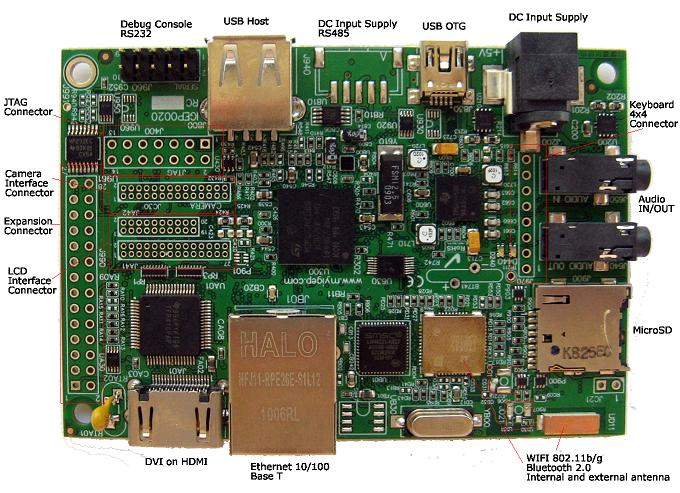
\includegraphics[width=\textwidth]{afbeeldingen/IGEPv2}
	\caption{IGEPv2}
\end{figure}

Dat hebben we gevonden in de vorm van de \strong{\makeurl{http://www.globalscaletechnologies.com/t-guruplugdisplaydetails.aspx}{GuruPlug Display}}. Deze computer is misschien minder krachtig (vooral acceleratiemogelijkheden zijn een prominente afwezige), maar wordt geleverd als een sluitend geheel waarbij het standaardpakket tevens voorziet van alle nodige kabels.

\begin{figure}
	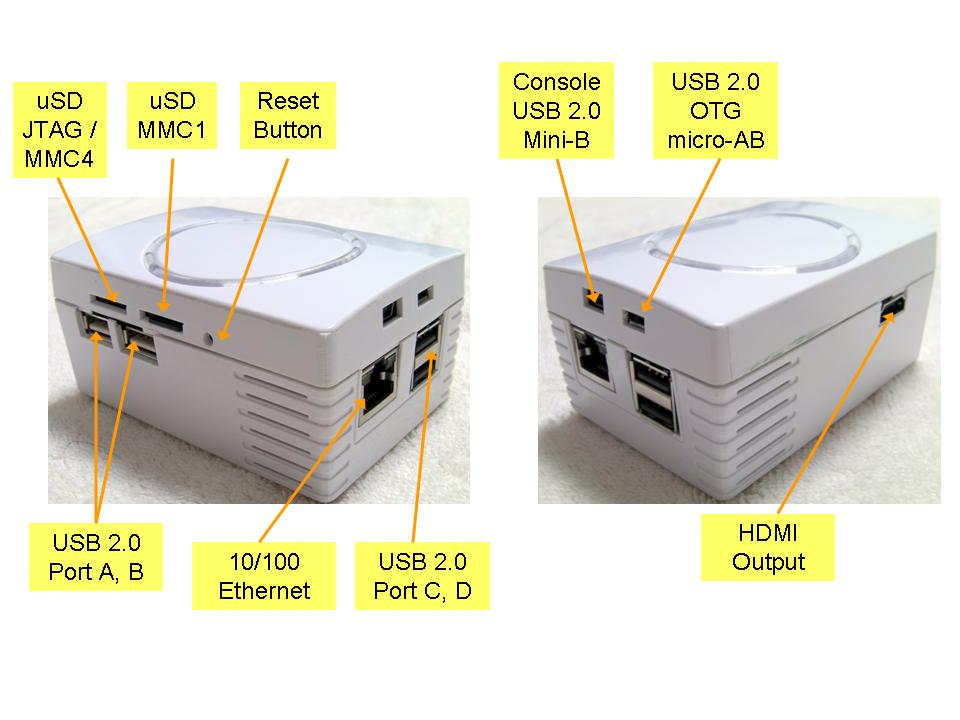
\includegraphics[width=\textwidth]{afbeeldingen/GuruPlug_Display}
	\caption{GuruPlug Display}
\end{figure}


\section{Interface module}
\label{ontwerp:hardware:interface}

De gebruikersinterface wordt gerealiseerd door 4 grote drukknoppen ingebouwd in de kast van elke kiosk. Momenteel worden deze knoppen intern doorverbonden met een afstandsbediening, waardoor de gebruiker via het indrukken van de knoppen indirect de DVD-speler kan besturen om zo een fragment te selecteren.

\begin{figure}
	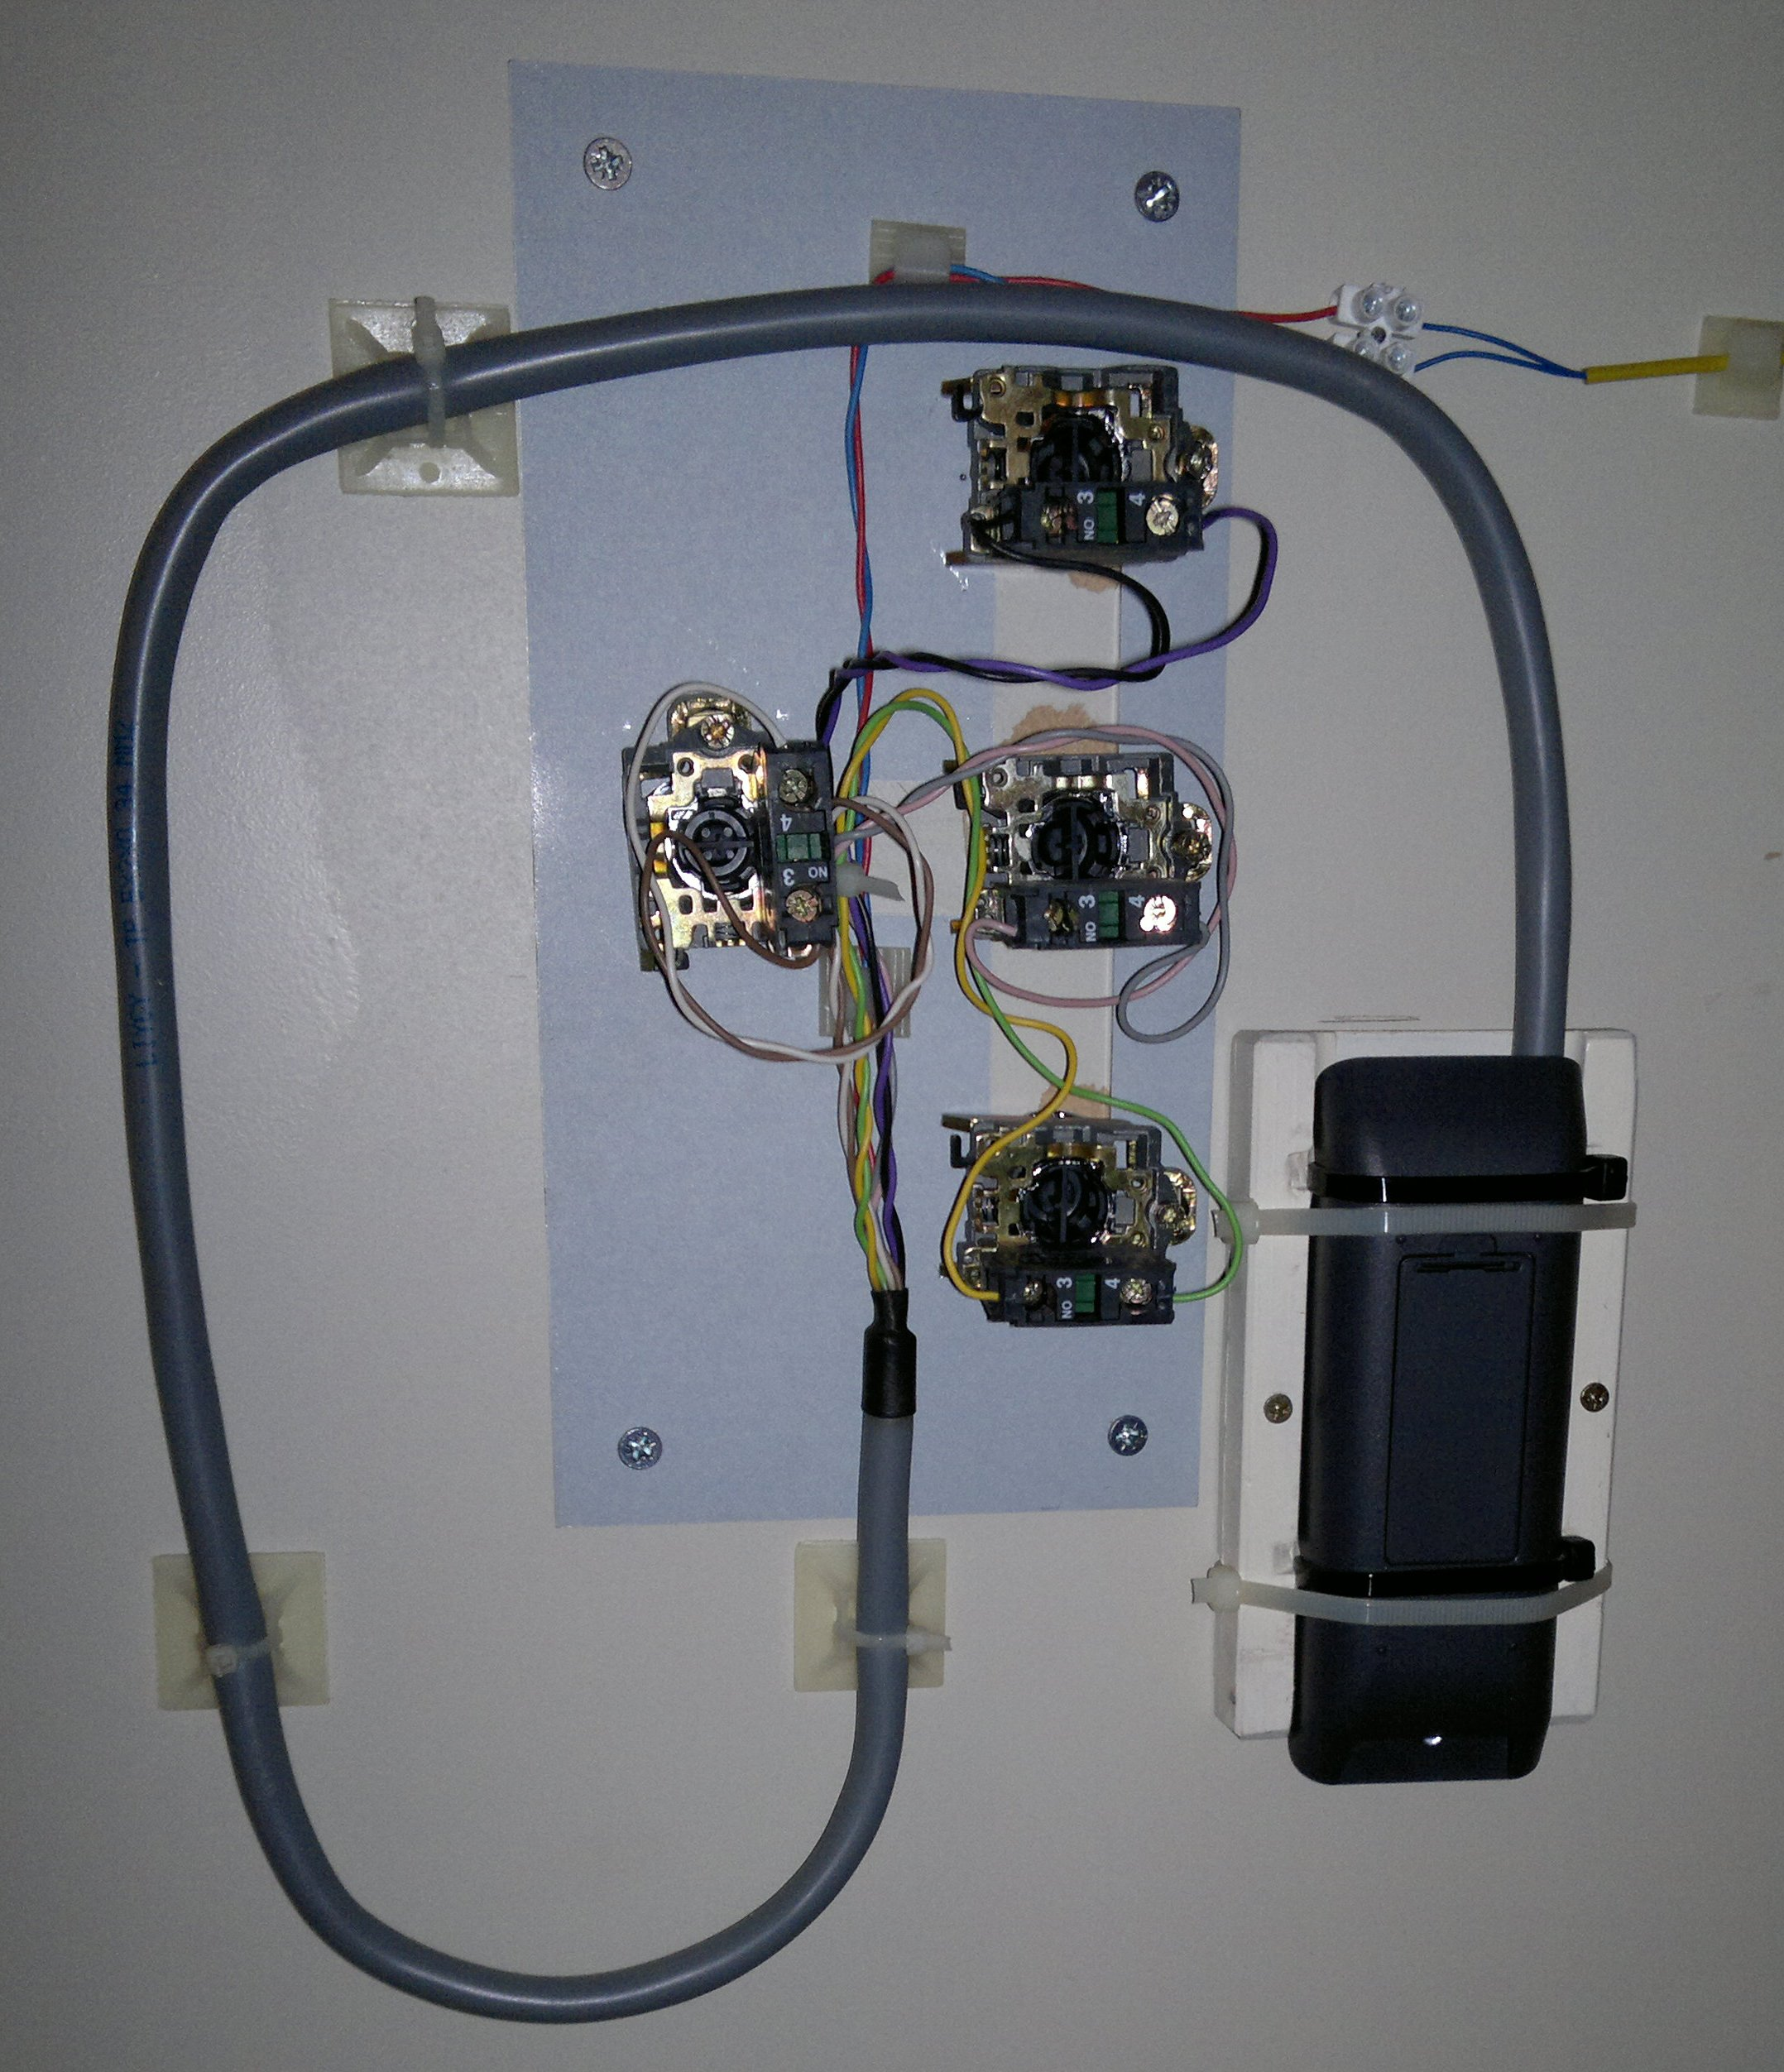
\includegraphics[width=\textwidth]{afbeeldingen/kiosk_knoppen}
	\caption{Huidige aansluitingsmethode knoppen}
\end{figure}

Nu we echter de DVD-spelers gaan vervangen door een computer, zullen we ook voor deze interface module een compatibel alternatief moeten vinden. Aan deze module worden enkele specifieke eisen gesteld:
\begin{itemize}
\item Goedkoop: de module moet zo goedkoop mogelijk te produceren zijn, alsook mag het niet teveel energie verbruiken;
\item Toekomstgericht: aansluitmogelijkheden mogen geen gebruik maken van oude protocollen;
\item Gebruiksvriendelijk: installatie van de module moet eenvoudig zijn;
\item Snel: de tijd tussen het indrukken van een toets en registratie van het signaal moet minimaal zijn;
\item Uitbreidbaar: het moet mogelijk zijn om later extra toetsen aan te sluiten.
\end{itemize}

\subsection{Aansluiting}

Het grootste ontwerpprobleem hierbij is de manier van aansluiting die we zullen gebruiken om de module in verbinding te brengen met de rest van de kioskhardware. De meeste eenvoudige keuze zou die zijn van de \strong{parallelle poort}, waarbij we de pinnen van de poort vrijwel direct zouden kunnen verbinden met de knoppen. Jammer genoeg zijn parallelle poorten steeds schaarser, en komt die vrijwel nooit meer voor op embedded hardware. Een andere toegankelijke optie is de \textbf{seriële poort}. Hierbij zou dan extra periferie benodigd zijn om in te staan voor de serialisatie van de signalen. Indien we echter platform-specifieke code toelaten, kunnen we de stuursignalen van de poort op een parallelle manier misbruiken zodat ook die periferie geëlimineerd wordt. Toch voldoet ook deze oplossing niet: ook de seriële poort wordt steeds schaarser, en alhoewel ze momenteel nog te vinden is op de meeste embedded-hardware bestaat de mogelijkheid dat dit binnen geringe tijd niet meer zo is.

Daarom hebben we uiteindelijk gekozen voor een poort die we normaal gezien wel nog enkele jaren zullen terugvinden op de meest courante hardware: de \ac{usb} poort. Deze veelzijdige poort laat ons doe om de interface module te laten communiceren met een computer, en is ook relatief toekomstgericht (de recent geïntroduceerde \ac{usb} versie 3 is nog steeds volledig terugwaarts compatibel met \ac{usb} versie 1 toestellen). Maar het gebruik van \ac{usb} kent ook een nadeel: het protocol is immers pakket-georiënteerd, waardoor extra periferie een noodzaak is. Ook is de configuratie complexer, zeker indien we een toestel willen dat zonder speciale stuurprogramma's werkt op verschillende besturingssystemen.

\subsection{Realisatie \acs{usb}-communicatie}

Aangezien \ac{usb} een pakket-georiënteerd protocol is, hebben we steeds extra periferie nodig om de gebruikersinvoer door te sturen. Om geen speciale software te vereisen moet onze module een apparaat uit de \ac{usb} \ac{hid} klasse implementeren. Voor bepaalde subcategorieën van deze klasse (zoals toetsenborden, muizen, \dots) wordt immers gegarandeerd dat compatibele besturingssystemen er mee zullen kunnen omgaan zonder daarvoor extra stuurprogramma's nodig te hebben. Daarom zullen we onze module zichzelf laten identificeren als een toetsenbord, waarbij we dan in de Javascript code van de voorstellingen gepast kunnen reageren op dergelijke toetsaanslagen.

Om een \ac{usb} toetsenbord te realiseren, zijn we in eerste instantie op zoek gegaan naar \strong{\ac{usb} keyboard encoders}. In de huidige opzet hebben we echter maar nood aan 4 knoppen, terwijl de meeste keyboard encoders veel meer toetsen toelaten. Daarom is de prijs meestal ook een pak hoger, zo kost de \makeurl{http://www.ultimarc.com/ipacve.html}{I-Pac VE} keyboard encoder, die 32 toetsen toelaat, reeds \$35!

Daarom lijkt het interessanter om zelf te voorzien in de conversie naar \ac{usb}-pakketten, door gebruik te maken van een \strong{microcontroller met \ac{usb} hardware}. Dergelijke microcontrollers voorzien in on-chip \ac{usb} communicatiemogelijkheden, net zoals de meeste reguliere microcontrollers toelaten om gegevens over een seriële \ac{uart} te transporteren. Om vervolgens de \ac{usb} hardware op een toegankelijke manier te gebruiken, bestaan er verschillende bibliotheken zoals de officiële \ac{usb} bibliotheek van Atmel, of het open-source \makeurl{http://www.fourwalledcubicle.com/LUFA.php}{\ac{lufa}}. Het nadeel van deze piste is echter de meerkost van de \ac{usb} hardware, die eigenlijk onnodig is daar we enkel gebruik zullen maken van de \emph{low speed} overdrachtsmodus.

Een derde optie is om gebruik te maken van een \strong{microcontroller met \ac{usb} software}. Hierbij hebben we geen speciale hardware nodig, enkel een microcontroller die krachtig genoeg is om de \ac{usb} software uit te voeren. Het grote nadeel hieraan is dat het met de huidige microcontrollers enkel mogelijk is om gebruik te maken van \emph{low speed} \ac{usb}, maar voor onze toepassing is dit geen probleem. Opnieuw zijn er verschillende mogelijkheden om dit te realiseren, waarvan er een beschreven is in een \makeurl{http://www.atmel.com/dyn/resources/prod\_documents/doc2556.pdf}{application note} van Atmel. Deze application note gebruikt relatief weinig hardware om elementaire \ac{usb} communicatie te realiseren, maar zoals later zal blijken zijn er zelfs nog efficiëntere configuraties mogelijk. Ook is de software geschreven in AVR assembler, waardoor het geheel niet zo overdraagbaar is. Daarom zullen we gebruik maken van een open-source alternatief: de \makeurl{http://www.obdev.at/products/vusb/index.html}{V-USB} bibliotheek. Deze in C-geschreven bibliotheek biedt een eenvoudigere interface en daarbij ook verschillende voorbeeldprojecten om het gebruik ervan te illustreren.

\end{document}

\part{Server}
\label{server}

% somehow grootorde/duur/sloc project integreren

\chapter{Structuur}

Op het hoogste niveau hebben we de serverapplicatie onderverdeeld in enkele logische subsystemen, zijnde het netwerk en de repository. Onderling communiceren deze subsystemen niet met elkaar: coördinatie verloopt door een overkoepelende controller. Zo is het mogelijk om elk subsysteem als een alleenstaand geheel te behandelen, wat het ontwikkelingsproces sterk vereenvoudigt. Tenslotte is er nog de webinterface, die dezelfde visibiliteit heeft als de controller: acties die een gebruiker uitvoert op de beheersinterface kunnen een impact hebben op objecten binnen het netwerk of de repository.

Om code te abstraheren en controle van subsystemen te vereenvoudigen moet elk van de subsystemen een bepaalde klasse uitbreiden met de concrete implementatie. Die klasse voorziet niet alleen in bepaalde gedeelde functionaliteit (zoals het genereren van log berichten, of inladen van de nodige configuratiebestanden), maar schrijft ook voor hoe de effectieve implementatie moet gevormd worden. Hierdoor wordt het eenvoudig om vanuit de applicatiecontroller op een eenduidige manier bepaalde standaardacties (zoals het opstarten of afsluiten van een subsysteem) uit te voeren.

\section{Netwerk subsysteem}

Het netwerk subsysteem verzorgt wat we in de vorige hoofdstukken tot applicatieprotocol gedoopt hebben. Het subsysteem is opgesplitst in enkele samenwerkende componenten: vooreerst is er het gedeelte dat dient als main entrypoint voor andere componenten die willen gebruik maken van het netwerksubsysteem. Daartoe biedt het bijvoorbeeld een lijst van aanwezige kiosken, en kan voor elke kiosk een object opgevraagd worden dat toelaat om gegevens op te halen of acties uit te voeren. Ook is er voorzien in de nodige functionaliteit om signalen door te geven, bijvoorbeeld om geschikt te reageren op de toevoeging van een nieuwe kiosk.
Door al deze functionaliteit te bundelen in een enkele klassie, is dit de enige interface tussen het volledige subsysteem en de rest van de applicaties. De uiteindelijke implementatie van het subsysteem kan hierdoor eenvoudig gewijzigd worden, zonder veel te moeten veranderen aan componenten die gebruik maken van dit systeem.

Het netwerk subsysteem bevat ook nog een gedeelte dat instaat voor de effectieve monitoring van het netwerk, door te reageren op signalen van de achterliggende \ac{upnp} bibliotheek. Dit gedeelte is puur intern, en het is niet de bedoeling dat een externe component communiceert met deze netwerk monitor. Als de monitor bepaalde informatie wil vrijgeven aan de buitenwereld (wat bijvoorbeeld voorkomt als het een nieuwe kiosk detecteerd), zal het dit doorgeven aan de publieke component van het netwerk subsysteem, waarna die bijvoorbeeld bepaalde signalen zal uitsturen. Hoewel dit geconvolueerd mag lijken is dit een hele interessant design: zoals hierboven vermeld mogen we nu steeds de monitor naar believen aanpassen, zolang de publieke interface maar dezelfde blijft zal niemand hier iets merken.

Om het voor de buitenwereld eenvoudig te maken om te interfacen met het netwerk, zal de publieke interface niet alleen informatie vrijgeven maar ook toegang bieden tot functionele objecten die eenvoudige manipulatie van hun onderwerp toelaten. Zo zal een \code{Network::getDevice(String uuid)} aanroep niet louter informatie over het toestel teruggeven, maar een volwaardig \code{Device} object. Dit object kan dan gebruikt worden om het toestel zelf te manipuleren: indien we bijvoorbeeld over een kiosk spreken zal eer voorzien zijn van een \code{Device::Shutdown} methode.

\section{Repository subsysteem}

Dit systeem dient als wrapper rond de repository waarbinnen alle gegevens van het systeem (configuraties en voorstellingen) opgeslagen zijn. Zoals vermeld in hoofdstuk \ref{ontwerp} staat de server in voor het ophalen en verwerken van de configuratiegegevens, en moet het de nodige kiosken laten weten wanneer de media die ze tonen gewijzigd is.

Net zoals bij het netwerk subsysteem biedt het repository subsysteem een publieke interface die de buitenwereld toelaat gegevens op te vragen. Ook zullen de teruggegeven objecten opnieuw gesofisticeerd zijn om eenvoud verwerken van de gegevens toe te laten: de \code{Repository::getConfiguration(String id)} aanroep bijvoorbeld zal daarom een \code{KioskConfiguration} object teruggeven dewelke specifieke functies bevat zoals \code{getVolume}. Hoewel dit systeem zijn nadelen kent -- een wijziging van het configuratieformaat vereist direct wijzigingen aan de servercode -- zorgt de rigide opzet ervoor dat inconsistenties tussen de repository en de achterliggende logica snel zullen duidelijk worden. 

Bij het opstarten van het repository subsysteem zal een initiële \code{checkout} uitgevoerd worden. Hierna zal een interne timer gestart worden die om de minuut controleert of er geen nieuwe revisie in de repository te vinden is. Indien dat het geval is, zullen alle configuraties opnieuw binnengehaald worden om dan eventueel de wijzigingen naar een client te sturen. Momenteel gebeurt dit echter vrij inefficiënt: alle configuraties worden opnieuw opgehaald en verstuurd, los van het feit of er ook effectief wijzigingen gebeurd zijn. Voor een volgende versie streven we ernaar om ook effectief de delta-gegevens te interpreteren en zo intelligent de nodige veranderingen door te sturen.

\section{Applicatiecontroller}

Dit systeem staat in voor de coördinatie van acties die niet geïsoleerd blijven tot een enkel subsysteem. Het beste voorbeeld hiervoor is voor wanneer het netwerk subsysteem een nieuwe component detecteert. Om de code overzichtelijk te houden zal het netwerk subsysteem dan geen actie ondernemen, maar louter zijn gegevens updaten en een signaal uitsturen. De applicatiecontroller vangt vervolgens dit signaal op om vervolgens de repository te raadplegen voor eventuele configuratiegegevens.

\section{Website subsysteem}

Deze component visualiseert de gegevens uit de repository en netwerk subsystemen, en laat de gebruiker toe om er controle over uit te oefenen. Die controle is echter beperkt: persistente configuratie moet nog altijd verlopen via manuele interventie.

\chapter{Besturingssysteem}

% todo

\chapter{Deployment}

\section{Buildsystem}

Voor het bouwen van een executable hebben we berust op \ac{maven}, een softwarebeheersysteem dat op een flexibele manier toelaat om alle aspecten van het bundelen van een applicatie te organiseren. Daartoe voorzien we in een \ac{pom} bestant waarin alle informatie verwerkt zit, zoals de naam en versie van de toepassing, de libraries waarop het berust, en hoe de applicatie moet opgestart worden. Aan de hand van die informatie kan \ac{maven} het project gepast uitvoeren of bundelen tot een finale executable.

Ook wordt het gebruik van externe libraries vereenvoudigt: er bestaat een \ac{maven} repository met daarin de meest populaire libraries, waardoor we louter de naam en versie in het \ac{pom} bestand moeten specificeren en \ac{maven} met deze informatie zelf op zoek gaat naar de gepaste binaries die benodigd zijn om de applicatie op te starten (zie bijvoorbeeld fragment \ref{lst:maven}).

\begin{lstlisting}[language=XML, float, caption=Inladen van externe libraries via Maven., label=lst:maven]
<dependencies>
  <dependency>
    <groupId>log4j</groupId>
    <artifactId>log4j</artifactId>
    <version>1.2.16</version>
  </dependency>
  ...
</dependencies>
\end{lstlisting}

Voor enkele libraries die we niet terugvonden in de officiële \ac{maven} repositories hebben we ofwel een alternatieve repository toegevoegd die het pakket wel bevatte (zoals dat was in het geval van Cling), of zelf voorzien in een lokale repository die de benodigde bestanden bevat en gebundeld is met de broncode om iedereen toe te laten de applicatie zonder al te veel moeite te compileren.

Ook kent \ac{maven} een plugin-systeem, dat we dankbaar gebruiken om bepaalde specifieke taken uit te voeren. Zo willen we bijvoorbeeld een \ac{jar} bestand genereren dat tegelijk alle afhankelijke libraries bevat, om zo installatie op de uiteindelijke server te vereenvoudigen. Dit druist deels in tegen de ideale manier om software te packagen, waarbij externe libraries steeds via de lokale package-manager geïnstalleerd worden, maar omdat we daarvoor zeer nauwgezet het pakket zouden moeten onderhouden (updates van een externe library kan immers steeds problemen veroorzaken in de applicatie zelf) hebben we ervoor gekozen om alles tesamen te bundelen tot een monolitisch geheel. Specifiek voor de serverapplicatie is de relevante configuratie daarvoor te vinden in fragment \ref{lst:fatjar}.

\begin{lstlisting}[language=XML, float, caption=Gebruik van Maven modules om een executable te compileren., label=lst:fatjar]
<build>
  <plugins>
    <plugin>
    <groupId>org.apache.maven.plugins</groupId>
    <artifactId>maven-assembly-plugin</artifactId>
    <executions>
      <execution>
        <id>package-jar-with-dependencies</id>
        <phase>package</phase>
        <goals>
          <goal>single</goal>
        </goals>
        <configuration>
          <appendAssemblyId>false</appendAssemblyId>
          <descriptorRefs>
            <descriptorRef>
              jar-with-dependencies
            </descriptorRef>
          </descriptorRefs>
          <archive>
            <manifest>
              <mainClass>
                be.mira.adastra3.server.Main
              </mainClass>
            </manifest>
          </archive>
        </configuration>
      </execution>
    </executions>
  </plugin>
</build>
\end{lstlisting}

% todo: debian packaging

\section{Webserver}

Zoals uitvoerig beschreven in hoofdstuk \ref{ontwerp} hebben we wegens het gebrek aan een serverside \ac{svn} library voor de server nood aan een externe \ac{svn} instantie. Om het beheer van zowel de serverapplicatie als die \ac{svn} instantie eenvoudig te houden, gaan we beide overkoepelen door een Apache webserver.

De eerste daarbij is de configuratie van een \ac{svn} instantie. Hierbij is het van belang dat enkel een beheerder die data kan wijzigen, maar iedereen er toegang tot heeft (er is geen nood aan authenticatie, de voorstellingen bevatten geen gevoelige data). Na het aanmaken van een \ac{svn} repository op de server kunnen we die overkoepelen door de Apache webserver via de configuratie uit fragment \ref{lst:apache:svn}.

\begin{lstlisting}[language=ApacheConfig, caption=Configuratie van Apache om een \ac{svn} server te overkoepelen., label=lst:apache:svn]
<Location "/repository">
  DAV svn
  SVNPath /var/db/subversion
  AuthType Basic
  AuthName "Ad-Astra III - Repository"
  AuthUserFile /etc/httpd/conf/repository.htpasswd
  Order deny,allow
  <LimitExcept GET PROPFIND OPTIONS REPORT>
    Require valid-user
  </LimitExcept>
</Location>
\end{lstlisting}

Vervolgens moeten we nog de beheersinterface van de serverapplicatie overkoepelen. Hierbij configureren we de embedded Tomcat instantie eerst om toegankelijk te zijn via het \ac{ajp} protocol, wat we op eenvoudige manier mogelijk gemaakt hebben via het standaard configuratiebestand dat met de broncode van de serverapplicatie geleverd wordt. Daarnaast moeten we er Apache op wijzen dat requests op een bepaalde locatie nog moeten doorgestuurd worden naar een externe applicatie. Dit gebeurt via de Apache Tomcat connector, te vinden in \code{mod\_jk}. Zoals te zien is in de Apache configuratie van fragment \ref{lst:apache:jakarta} wordt daarbij nog verwezen naar een extern bestand: dit bevat de configuratie die \code{mod\_jk} nodig heeft om de externe applicatie bereiken, namelijk de locatie van de applicatie en hoe ermee moet gecommuniceerd worden (zie fragment \ref{lst:jakarta}).

\begin{lstlisting}[language=ApacheConfig, float, caption=Configuratie van Apache om een externe Jakarta applicatie te overkoepelen., label=lst:apache:jakarta]
// Inladen van de connector
LoadModule jk_module modules/mod_jk.so

// Specificeren van het configuratiebestand
JkWorkersFile /etc/httpd/conf/jakarta.properties

// Instellen van de logging
JkShmFile        /var/log/httpd/mod_jk.shm
JkLogFile        /var/log/httpd/mod_jk.log
JkLogLevel       info
JkLogStampFormat "[%a %b %d %H:%M:%S %Y] "

// Doorverwijzen van een bepaalde locatie
JkMount /status/* worker1
\end{lstlisting}

\begin{lstlisting}[language=JavaProperties, float, caption=Configuratie van de Apache Tomcat connector., label=lst:jakarta]
# Registreren van alle workers
worker.list=worker1

# Configureren van een worker
worker.worker1.type=ajp13
worker.worker1.host=localhost
worker.worker1.port=8009
\end{lstlisting}
\part{Kiosk}
\label{kiosk}

\chapter{Structuur}

De manier waarop we de kioskapplicatie hebben opgedeelt kent sterke gelijkenissen met de manier waarbij we de serverapplicatie gestructureerd hebben: alle logische componenten (de networkinterface, de userinterface en de datamanager) worden geïsoleerd in een apart subsysteem, en een overkoepelende controller staat in voor interacties die over verschillende subsystemen heen gaan.

\section{Network interface}

Dit gedeelte van de applicatie neemt alle netwerkcommunicatie op zich. Daartoe creëert het een \ac{upnp} device, registreert het de nodige services, en broadcast het die gegevens. Wanneer een bepaalde actie aangeroepen wordt, zal de respectievelijke service louter een signaal uitsturen. Dat signaal (bijvoorbeeld \code{reboot} of \code{setVolume(uint)}) zal vervolgens opgevangen worden door de applicatiecontroller, die dan tot de effectieve actie overgaat.

Door de effectieve implementatie in een andere klasse te plaatsen vereenvoudigen we de netwerkinterface die in de minimale opzet al complex genoeg is (beheren van \ac{upnp} state variables, conversie van parameters, registratie van \ac{scpd} bestanden, \ldots). Tevens wordt de hele component hierdoor platform-onafhankelijk, en moeten we bij het herimplementeren voor een nieuw platform enkel de implementatie herschrijven die volledig geïsoleerd is binnen de applicatiecontroller. Dit is opnieuw vergelijkbaar met de opzet die we gehanteerd hebben bij de serverapplicatie: code binnen een bepaald subsysteem staat enkel in voor verwerking relevant toe dat subsysteem, acties die ergens anders een impact hebben worden afgehandeld door de applicatiecontroller.

\subsection{Datamanager}

Deze klasse komt overeen met het repository subsysteem in de serverapplicatie, maar heeft een andere naam gekregen wegens een \emph{namespace clash} met enkele klassen die we gebruiken uit een library. De taken veranderen echter niet: de datamanager staat in  voor het ophalen van gegevens die zich in een externe \ac{svn} repository bevinden, en alles dat daarmee gepaar gaat. Zo zal de component moeten rekening houden met een eventuele cache, om zo een checkout van gegevens te versnellen. Ook moet het bij het opstarten kunnen controleren of er geen oude checkout aanwezig is, om zo direct al een voorstelling te kunnen weergeven, zelfs als dat een oude voorstelling betreft.

In tegenstelling tot de repository klasse in de serverapplicatie moeten we hier geen data interpreteren: na een checkout of update gedaan te hebben, moet de voorstelling in zijn geheel opnieuw doorgegeven worden aan de userinterface, het is niet van belang om te weten wélke gegevens veranderd zijn. Hierdoor wordt het gebruik van de \ac{svn} libraries sterk vereenvoudigt.

\subsection{Userinterface}

Dit gedeelte van de applicatie staat in voor de effectieve weergave van ontvangen voorstellingen. Zoals reeds vermeld bestaan die voorstellingen uit \ac{html} en Javascript, en gebruiken we de WebKit rendering engine om die gegevens weer te geven. In de huidige opzet hebben we enkel voorzien in een naadloze integratie van de rendering engine en onze applicatie, waardoor de voorstellingen zeer vlot geladen en verwerkt kunnen worden. Voor een volgende versie plannen we deze component uit te breiden zodat het niet alleen voorstellingen weergeeft, maar gegevens over hoe exact die weergegeven worden teruggestuurd worden naar de server. Zo kunnen we bijvoorbeeld statistieken vergaren over welke voorstellingen het meest bekeken worden, welke filmpjes het snelst gestopt worden, \ldots

Omdat de integratie van de rendering engine en de rest van de applicatie zo goed bleek te werken, hebben we besloten om de overige gebruikersinterfaces op eenzelfde manier te implementeren in \ac{html} en Javascript. Hoewel er niet zoveel reguliere interfaces binnen de applicatie te vinden zijn (opstart-pagina, en enkele debug pagina's), resulteerde dit in een uniforme userinterface-implementatie waarbij het zelf op termijn mogelijk zou moeten zijn om de interface code dynamisch te updaten op eenzelfde manier als dat bij de voorstellingen gebeurt.

Er is echter een groot verschil tussen een ordinaire voorstelling en een userinterface-pagina bij de applicatie: waar een voorstelling volledig \emph{self-contained} is, heeft een informatieve userinterface-pagina gegevens nodig uit de applicatie. Een debugpagina bijvoorbeeld heeft nood aan een mechanisme om debuggegevens van de applicatie te ontvangen.
Een mogelijkheid zou zijn om via \ac{ajax} gegevens op te halen die via een webservice lokaal opengesteld worden. Dit verhoogt echter de complexiteit van zowel de interface als de kioskapplicatie, laat staan dat het een efficiënte manier is om een weinig gegevens over te brengen. Daarom hebben we gekozen voor een secundaire piste, waarbij we gebruik maken van de \makeurl{http://doc.qt.nokia.com/latest/qtwebkit-bridge.html}{QtWebKit Bridge}. Dit mechanisme laat ons toe om een klasse binnen onze C++ applicatie toegankelijk te maken vanuit Javascript code, om zo gegevens op een efficiënte manier te kunnen doorspellen. Zo hebben we voor alle soorten pagina's die we moeten kunnen weergeven, een meta-klasse aangemaakt die de nodige gegevens aggregeert (zie fragment \ref{lst:expose_cpp}). Bij het aanmaken van de pagina in kwestie wordt die meta-klasse vervolgens geregistreert binnen de rendering engine, waardoor de Javascript code die met de pagina geladen wordt er toegang tot heeft. Een voorbeeld van dit laatste is te zien in fragment \ref{lst:expose_js}.

\begin{lstlisting}[language=C++, float, caption=Registratie van een klase binnen de rendering engine., label=lst:expose_cpp]
class LogPage : public QWebPage
{
Q_OBJECT
Q_PROPERTY(QString id READ id CONSTANT)
public:
    LogPage(QObject* parent = 0);
    ~LogPage();

    QString id() const;
signals:
    void newMessage(const QString& iMessage);
};

LogPage::LogPage(QObject *parent) : QWebPage(parent)
{
    mainFrame()->addToJavaScriptWindowObject(
    	"application",
        this);
}
\end{lstlisting}

\begin{lstlisting}[language=JavaScript, float, caption=Gebruik van een geregistreerde C++ klasse., label=lst:expose_js]
// Gebruik van een signaal
function showMessage(message)
{
	...
}
application.newMessage.connect(showMessage);

// Gebruik van een property
document.write(application.id)
\end{lstlisting}


\chapter{Realisatie}

Tijdens de realisatie van de kioskapplicatie zijn we op enkele interessante problemen gestuit die zeker het vermelden waard zijn.

\section{Uniek ID}

Aangezien de software die op de kiosken zal draaien volledig identiek is -- we streven immers naar een configuratieloze opzet -- moet de applicatie in staat zijn om een identifier te genereren die uniek is, maar toch gebonden aan een specifieke kiosk om er vanuit de configuratie naar te kunnen verwijzen. De identifier zal gebruikt worden door de \ac{upnp} library, die het doorspeelt naar een externe partij als deel van de device description. Daarom zullen we ons moeten schikken naar de \ac{upnp} standaard, die een \ac{uuid} vereist als identifier.

Een \ac{uuid} is zeer specifiek opgemaakt, en bestaat steeds uit 16 bytes, onderverdeeld in 5 groepen die elk gescheiden zijn door een steepje: \code{DEADBEEF-E29B-41D4-A716-446655440000}. Er bestaan echter verschillende \ac{uuid} varianten, elk met een aantal versies. Zowel de variant als de versie wordt in de \ac{uuid} string geëncodeerd, met als template \code{xxxxxxxx-xxxx-Mxxx-Nxxx-xxxxxxxxxxxx}. De officiële specificatie detailleert maar 1 variant, die geïdentificeerd wordt door de twee meest-significante bits van de \code{N} byte op $1 0$ in te stellen. Betreffende de versie hebben we de keus uit een aantal versies, en kiezen we voor een gewijzigde vorm van de \ac{mac} versie. Hierbij moet de \code{M} byte ingesteld worden op een hexadecimale 1, en kunnen we de eerste twee groepen (samen exact 12 bytes) gebruiken om het \ac{mac} adres in te encoderen.

Normaal worden de overige bits vervolgens gevuld met tijdsgegevens, maar omdat we willen dat onze identifier identiek blijft na een reboot kiezen we ervoor om die bits op 0 in te stellen. Het resultaat hiervan valt te vinden in fragment \ref{lst:uuid}.

\begin{lstlisting}[language=C++, float, caption=Generatie van een \ac{uuid}., label=lst:uuid]
QUuid getHardwareUuid() const
{
  // Maak een interface request object aan
  struct ifreq tRequest;
  bzero(&tRequest, sizeof(tRequest));
  tRequest.ifr_addr.sa_family = AF_INET;
  strncpy(tRequest.ifr_name, "eth0", IFNAMSIZ-1);

  // Open een socket en voer de systeemaanroep uit
  int tFd = socket(AF_INET, SOCK_DGRAM, 0);
  ioctl(tFd, SIOCGIFHWADDR, &tRequest);
  close(tFd);

  // Genereer een UUID
  char* tMAC = ifr.ifr_hwaddr.sa_data
  QUuid oUuid;
  oUuid.data1    |= (unsigned char) tMAC[0] << 24;
  oUuid.data1    |= (unsigned char) tMAC[1] << 16;
  oUuid.data1    |= (unsigned char) tMAC[2] << 8;
  oUuid.data1    |= (unsigned char) tMAC[3];
  oUuid.data2    |= (unsigned char) tMAC[4] << 8;
  oUuid.data2    |= (unsigned char) tMAC[5];
  oUuid.data4[0]  = (oUuid.data4[0] & 0x3F  ) | 0x80;
  oUuid.data3     = (oUuid.data3    & 0x0FFF) | 0x1000;
  
  return oUuid;
}
\end{lstlisting}

\section{BRisa \ac{upnp} library}

Zoals reeds vermeld gebruiken we de BRisa library aan de kant van de kiosk, waarbij acties en methodes opgeroepen worden door de Cling bibliotheek aan de kant van de server. Cling staat er echter voor bekend om de \ac{upnp} specificatie op de letter te volgen, waarbij elke afwijking daarvan als een waarschuwing of zelfs vaak als een regelrechte fout beschouwd wordt. En jammer genoeg bleek de BRisa bibliotheek soms laks om te gaan met de standaarden voorgeschreven door de \ac{upnp} standaard \ldots

Om Cling te overtuigen om zonder veel probleem te werken met clients die de BRisa bibliotheek gebruiken, hebben we twee patches moeten doorvoeren. De eerste daarvan introduceert een extra spatie voor het \code{s:encodingStyle} attribuut dat meegestuurd wordt bij elk \ac{soap} bericht. Zonder deze spatie weigerde Cling de antwoorden van de BRisa bibliotheek te verwerken, waardoor het onmogelijk een actie uit te voeren. Een tweede patch voegt de optionele \code{content-type} header toe aan berichten waarbij de ontwikkelaars van BRisa dat vergeten waren, waardoor Cling nu ook zonder waarschuwingen kan communiceren met een BRisa server.

Hierbij was het een groot voordeel dat de library open-source was. Nadat we het probleem gelocaliseerd hadden door de foutmeldingen van Cling te combineren met een analyse van de verzonden berichten, konden we eenvoudig de code van de library ophalen, het probleem localiseren en oplossen. Hoewel we beide patches ingestuurt hebben op de bug tracker van het BRisa project (\makeurl{https://garage.maemo.org/tracker/index.php?func=detail\&aid=6953\&group\_id=138\&atid=583}{eerste patch}, \makeurl{https://garage.maemo.org/tracker/index.php?func=detail\&aid=6954\&group\_id=138\&atid=583}{tweede patch}), kon het gerust nog even duren vooraleer de wijzigingen toegepast worden, of dat een nieuwe versie zou vrijgegeven worden. Daarom hebben we een \makeurl{https://github.com/MIRAvzw/qt-brisa}{onze eigen versie} van het project gemaakt (ook wel een \emph{fork}) genoemd, waarin de fouten reeds gecorrigeerd zijn. Op de toestellen waarop de applicatie ontwikkeld en geïnstalleerd wordt kunnen we nu in afwachting van een nieuwe versie onze eigen versie van de bibliotheek op installeren.

\section{svnqt \ac{svn} library}

Zoals beschreven in hoofdstuk \ref{ontwerp} hebben we voor onze kioskapplicatie een interessante \ac{svn} library gevonden die gebruik maakt en geïntegreerd is met het Qt framework dat we gebruiken. De code was oorspronkelijk een stand-alone library, genaamd ``svncpp" en ontwikkeld door RapidSVN in 2002. Nadien is de code geïntegreerd en verder ontwikkeld als deel van de KDESvn applicatie. Om de code eenvoudig doch efficiënt te kunnen gebruiken binnen onze kioskapplicatie hebben we code uit de KDESvn applicatie geëxtraheerd en er een \makeurl{https://github.com/MIRAvzw/svnqt}{alleenstaande bibliotheek} van gemaakt. Buiten enkele kleine wijzigingen hebben we niks moeten wijzigen om deze code vervolgens te kunnen gebruiken binnen ons project.

\section{Log4qt library}

Log4qt is een project dat een Log4J-achtige interface aanbiedt om op eenvoudige manier een consistente logging te voorzien, waarbij het mogelijk is om via een configuratiebestand de specifiëren waar de logberichten terechtkomen (zoals te zien is in fragment \ref{lst:log4qt}). Hoewel de bibliotheek functioneel vrij compleet is en op het eerste zicht geen problemen opleverde, hebben we naar verloop van tijd toch enkele wijzigingen toegebracht aan de \emph{upstream} code.

\begin{lstlisting}[language=JavaProperties, float, caption=Externe configuratie van Log4qt., label=lst:log4qt]
# Registreer alle appenders
log4j.rootLogger          = DEBUG, dbg

# Debug appender
log4j.appender.dbg        = org.apache.log4j.FileAppender
log4j.appender.dbg.file   = debug.log
log4j.appender.dbg.layout = org.apache.log4j.TTCCLayout
\end{lstlisting}

Een \makeurl{https://gitorious.org/log4qt/log4qt/merge\_requests/3}{eerste patch} die we ingestuurd hebben corrigeerde een probleem met namespaces. C++ code die gebruik maakt van Qt wordt immers eerst gepreprocessed door een Qt-specifieke preprocessor: de \ac{moc}. Deze preprocessor zorgt ervoor dat Qt meta-object en introspectiemogelijkheden krijgt, wat krachtige mechanismen zoals \code{signals \& slots} mogelijk maakt. Dit mechanisme is echter niet altijd even robuust: externe factoren kunnen ertoe leiden dat een \ac{moc}-macro verkeerd expandeert, en dat was hier het geval bij een ontbrekende namespace prefix binnen een \code{Q\_PROPERTY} \ac{moc}-macro.

Vervolgens hebben we ook enkele kleine features toegevoegd die het werken met de bibliotheek aangenamer maken. Zo hebben we voorzien in een \makeurl{https://gitorious.org/log4qt/log4qt/merge\_requests/4}{patch} die het mogelijk maakt om de Log4qt objecten te gebruiken met output operatoren: dit is een veelgebruikte techniek in de officiële Qt libraries waardoor de Log4qt bibliotheek eenvoudiger is voor mensen die er nog niet thuis in zijn maar toch ervaring hebben met Qt. Op vergelijkbare wijze hebben we de manier om headers te includen \makeurl{https://gitorious.org/log4qt/log4qt/merge\_requests/5}{gewijzigd} zodat het eveneens dichter aanleunt bij de manier waarop dat gebeurt bij de officiële Qt code.


\chapter{Deployment}

\section{Besturingssysteem}

% todo

\section{Compilatie}

Om de software te compileren maken we gebruik van de tools die het Qt framework daartoe biedt. De belangrijkste daarvanis \code{qmake}, een applicatie die het genereren van een \code{Makefile} automatiseert. Dit is vooral interessant omdat zoals hierboven vermeld bronbestanden die gebruik maken van Qt-macro's eerst moeten voorverwerkt worden door de \ac{moc} preprocessor. Door gebruik te maken van qmake moeten we dit niet langer manueel doen: qmake detecteert welke bestanden eerst moeten verwerkt worden door de preprocessor, en genereert een \code{Makefile} waarbij dit dan ook eerst gebeurt.

Ook hebben we tijdens de ontwikkeling van de applicatie gebruik gemaakt van \makeurl{http://clang.llvm.org/}{Clang}, een moderne compiler voor C en C++. Hoewel deze vrij jonge compiler nog niet op hetzelfde niveau staat als de \ac{gcc}, is het op enkele vlakken veel beter dan \ac{gcc}. Zo is er zeer veel aandacht besteed aan het error reporting subsysteem, waardoor de foutmeldingen die Clang genereert vaak een pak behulpzamer zijn dat wat \ac{gcc} in eenzelfde situatie zou laten weten. Toch worden de uiteindelijke executables gegenereert met \ac{gcc}, omdat die op vlak van optimalisaties (zowel op vlak van snelheid als grootte) nog steeds de beste keuze is.

\section{Packaging}

% todo: vermelden shared linken

% todo
\documentclass[verslag.tex]{subfiles} 
\begin{document}

\part{Interface module}
\label{interface}

\chapter{Hardware}

Zoals uit de doeken gedaan in deel \ref{ontwerp}, zullen we voor de interface gebruik maken van een AVR microcontroller met daarop de V-USB firmware om low speed datacommunicatie te verwezenlijken met minimale periferie.

\section{Microcontroller}

Door het gebruik van de V-USB bibliotheek moeten we ons beperken tot AVR microcontrollers, maar binnen die familie is het aanbod nog altijd zeer groot. Om een goede selectie te maken, moeten we logischerwijs rekening houden met de eisen die de V-USB bibliotheek stelt:
\begin{itemize}
\item Flash: tenminste 2 kB;
\item RAM: tenminste 128 bytes;
\item Kloksnelheid: 12.8 of 16.5 MHz bij gebruik van een interne oscillator, en ook 12, 15, 16 of 20 MHz indien we gebruik maken van een extern kristal\footnote{Dit omdat enkel de 12.8 en 16.5 MHz frequenties een deviatie van 1\% toelaten, en het bij een interen oscillator onmogelijk is om een heel precieze afstelling te bekomen.};
\item Poorten: exact 2, beide met een interruptlijn.
\end{itemize}

We willen echter ook een uitbreidbare module realiseren. Momenteel hebben we slechts 4 knoppen aan te sluiten, maar mogelijks worden dit er later meer. Daarom zullen we de ruimte laten voor drie extra knoppen, wat we eenvoudig kunnen realiseren met slechts 4 poorten door het signaal te multiplexen. Als we tenslotte overlappingen negeren, volstaat het zelfs om maar 3 poorten te gebruiken.

Tenslotte zou het ook interessant zijn moest de microcontroller voorzien van \ac{isp} headers, waardoor de firmware van de module achteraf nog kan vernieuwd worden zonder daarvoor de microcontroller te moeten verwijderen uit de module. Indien we het echter mogelijk willen maken om de chip te herprogrammeren via \ac{isp}, kunnen we geen gebruik maken van \ac{hvsp} (waarvoor de chip fysiek moet geplaatst in een \ac{hvsp} programmer moet geplaatst worden). \ac{hvsp} is een speciale methode om een microcontroller te programmeren, waarbij het mogelijk is om voordien ingestelde \emph{fuses} opnieuw in te stellen. Zo is er bijvoorbeeld de fuse die de \code{RESET}-poort (aanwezig op elke AVR microcontroller) configureert als een reguliere input/output poort. Deze fuse kan initieel wel ingesteld worden via \ac{isp}, maar heeft als consequentie dat de chip nadien niet meer kan geherprogrammeerd worden, tenzij door gebruik te maken van \ac{hvsp} waarmee de fuse in kwestie opnieuw ingesteld kan worden. Hierdoor is het dus onmogelijk om de \code{RESET}-poort te gebruiken als reguliere poort.

Een microcontroller die voldoet aan deze eisen, is de \strong{AtTiny45}. Deze heeft de volgende relevante specificaties:
\begin{itemize}
\item Flash: 4 kB;
\item RAM: 256 bytes;
\item EEPROM: 256 bytes;
\item ISP: aanwezig;
\item Kloksnelheid: 10 MHz voor de low-voltage versie, en tot 20 MHz voor de reguliere versie;
\item Interne oscillator: gekalibreerd voor 8 MHz;
\item Voedingsspanning: 1.8-5.5 volt voor de low-voltage versie, en 2.7-5.5 volt voor de reguliere versie.
\end{itemize}

\subsection{Kloksnelheid}

Om het aantal componenten te minimaliseren, zouden we de module graag realiseren zonder gebruik te maken van een externe oscillator. De interne oscillator is echter enkel gekalibreerd om op 8 MHz te werken, wat niet bruikbaar is in combinatie met V-USB. Om toch een bruikbare frequentie te bekomen, maken we gebruik van een kalibratiemechanisme terug te vinden in het \makeurl{http://www.obdev.at/products/vusb/easylogger.html}{EasyLogger} voorbeeldproject.

De eerste stap bestaat uit het kalibreren van de interne oscillator tot een frequentie van 8.25 MHz, dit door te vergelijken met binnenkomende \ac{usb} frames en binair te zoeken naar een optimale waarde voor het \code{OSCCAL} oscillator kalibratieregister. Hierdoor zal de \ac{pll} clock, steeds gelijk aan een achtvoudige versnelling van de interne oscillator, ingesteld worden op 66 MHz. Indien we tenslotte de \code{CLKSEL} fuse bij het programmeren instellen op $0001$ zal de systeemklok gelijk ingesteld worden aan de \ac{pll} clock gedeeld door 4, wat overeen komt met 16.5 MHz, een frequentie die we kunnen gebruiken in combinatie met de V-USB code.

\subsection{Voeding}

Aangezien de kloksnelheid waarop onze microcontroller zal draaien, 16.5 MHz, groter is dan 10 MHz, zullen we geen gebruik kunnen maken van de low-voltage versie. Meer nog: om een kloksnelheid groter dan 10 MHz te bekomen, zal de voedingsspanning zelfs tussen de 4.5 en 5.5 volt moeten bedragen. Op het eerste zicht vormt dit geen probleem, we kunnen immers de \ac{usb} voedingslijn (mits ontkoppeling) direct gebruiken om de microcontroller te voeden. Maar zoals uit de volgende paragraaf zal blijken, zou het zo ook zijn voordelen kennen moesten we de microcontroller kunnen voeden met een lagere spanning.

Natuurlijk zullen we ook de voedingsspanning ontkoppelen, en dit op twee vlakken. Om de hoogfrequente schakelpieken van de digitale microcontroller af te vlakken, plaatsen we een 100 nanofarad condensator tussen de voedingslijn en de grondplaat. Het valt op te merken dat we die condensator zo dicht mogelijk tegen de voedingspin van de microcontroller willen plaatsen, dit om parasitaire capaciteiten te vermijden. Vervolgens willen we ook eventuele ongerelmatigheden afvlakken (hetzij van de spanningsbron uit, hetzij veroorzaakt door een plotse toename in verbruik), waarvoor we een 10 microfarad condensator plaatsen aan de kant van de \ac{usb} connector. De waarde van 10 microfarad is niet uit de lucht gegrepen: ze is relatief hoog om de typisch laagfrequentere pieken die een spanningsbron genereert af te vlakken, en tegelijk is het ook het maximum dat de \ac{usb} specificatie \makeurl{http://www.beyondlogic.org/usbnutshell/usb2.shtml}{toelaat}.

\begin{figure}
	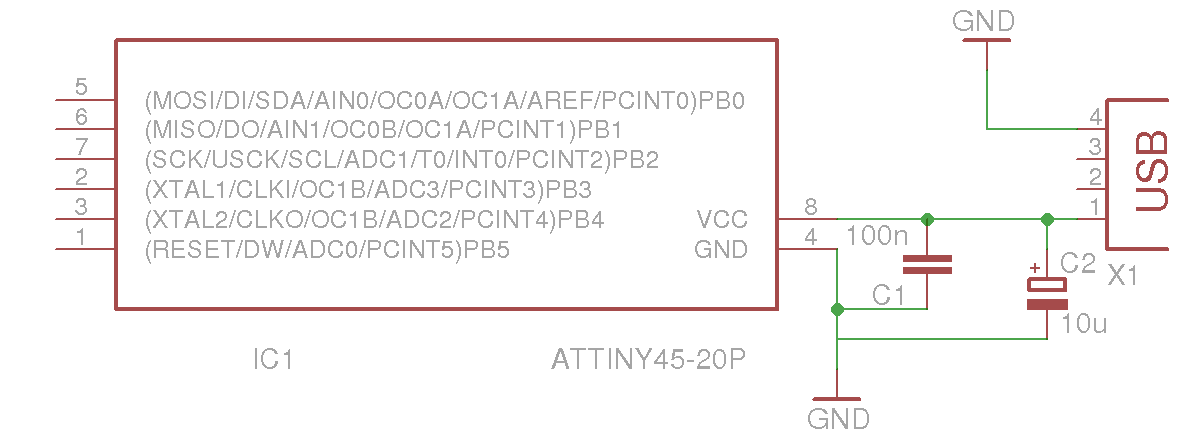
\includegraphics[width=\textwidth]{afbeeldingen/circuit_voeding}
	\caption{Voedingscircuit}
\end{figure}

\subsection{Signalen}

\ac{usb} datacommunicatie verloopt steeds over een \emph{twisted-pair}, op een differentiële manier. Dit betekent dat een signaalbit afgeleid wordt uit het potentiaalverschil tussen de twee signaaldragers, en dat die binnen een \ac{usb}-kabel steeds getwist zijn. Het voordeel van het twisten is dat eventuele ruis grotendeels evenredig verdeeld is over beide kabels, waardoor het potentiaalverschil tussen beide vaak onveranderd blijft. Hierdoor is differentiële dataoverdracht over een twisted-pair veel beter bestand tegen elektromagnetische ruis.

Eerst en vooral zorgen we voor een stroombeperking op de signaaldragers. Hiertoe zullen we tussen de signaalpin en de \ac{usb} connector een weerstand van 68 ohm plaatsen, die ervoor zorgen dat er nooit meer dan 50 milliampères zal vloeien.

De specifieke elektrische kenmerken van de implementatie in het \ac{usb} protocol zijn echter vervelend voor gebruik in combinatie met de meeste digitale componenten. Zo wordt een hoog signaal gekenmerkt door een differentieel signaal van 2.8 tot 3.6 volt, terwijl voor een laag signaal 0 tot 0.3 volt te detecteren valt. Voor toekomende signalen (het twisted-pair is immers half-duplex) vormen deze waarden geen probleem: de meeste microcontrollers, waaronder de gebruikte AtTiny45, herkennen een signaal van 3.3 volt als een hoog signaal (hoewel de specificatie slechts een bereik vastlegt, sturen de meeste hosts exact 3.3 volt) . Wat wel een probleem vormt, zijn de uitgaande signalen. Aangezien onze microcontroller gevoed wordt door 5 volt, kennen de signalen tevens een spanning van 5 volt, wat ruimschoots buiten het opgelegde bereik valt.

Een mogelijke oplossing bestaat eruit de \strong{voedingsspanning van de microcontroller te verlagen} tot 3.6 volt. Aangezien de spanning die de microcontroller gebruikt op de signaalpinnen min of meer gelijk is aan de voedingsspanning, en de AtTiny45 genoeg heeft aan slechts 1.8 tot 2.7 volt (afhankelijk van de uitvoering), zou dit het probleem direct oplossen. Er zou enkel nood zijn aan een spanningsregulator om de voedingsspanning te reduceren tot 3.6 volt, wat dan wel een \emph{low-drop} regulator zou moeten zijn (omdat gewone regulators meestal een initiële drop van 2 volt kennen). Een minder robuust vervangt deze regulator door twee diodes, waardoor een voltage drop van 1.2 tot 1.4 volt bekomen wordt.
Jammer genoeg kunnen we geen van deze oplossingen gebruiken, omdat de microcontroller op 16.5 MHz zal draaien waarvoor we een voedingsspanning tussen de 4.5 en 5 volt nodig hebben.

Een alternatief bestaat eruit om het \textbf{spanningsniveau van de signaalpinnen te reguleren}. Hiertoe raadt de \makeurl{http://vusb.wikidot.com/hardware}{V-USB wiki} bijvoorbeeld aan om gebruik te maken van 3.6 volt zenerdioden. Zenerdioden hebben immers de eigenschap dat ze, van zodra de zenerspanning bereikt is, in sper geleidt alsook dat de spanning erover relatief constant blijft. Meer concreet houdt dit in dat, indien we de signaalpinnen via een zenerdiode in sper verbinden met de grondplaat, de spanning van het signaal gereduceerd wordt tot 3.6 volt. Deze opzet kent echter ook enkele problemen. Zo kan het moeilijk zijn om de exacte combinatie van parameters vast te leggen, zenerdiodes komen immers in soorten en maten. Een ander nadeel zijn de hoge stromen veroorzaakt door de zenerdiode. Wanneer de diode immers een hoog 5 volt signaal reduceert tot 3.6 volt, zal de overige 1.4 volt over de 68 ohm weerstanden tussen de microcontroller en de \ac{usb} host komen te staan, wat zorgt voor liefst 20 milliampères over de signaaldrager.

Tenslotte moeten we nog voorzien in een \emph{setting weerstand} die een spanning plaatst op de negatieve signaaldrager. Deze pull-up weerstand maakt aan de \ac{usb} host duidelijk te maken dat er een \ac{usb} 1.1 toestel aangesloten is (weliswaar actief in \emph{low speed} modus). Voor een 5 volt lijn kan dit gerealiseerd worden met een 1k8 of 2k2 ohm weerstand.

\begin{figure}
	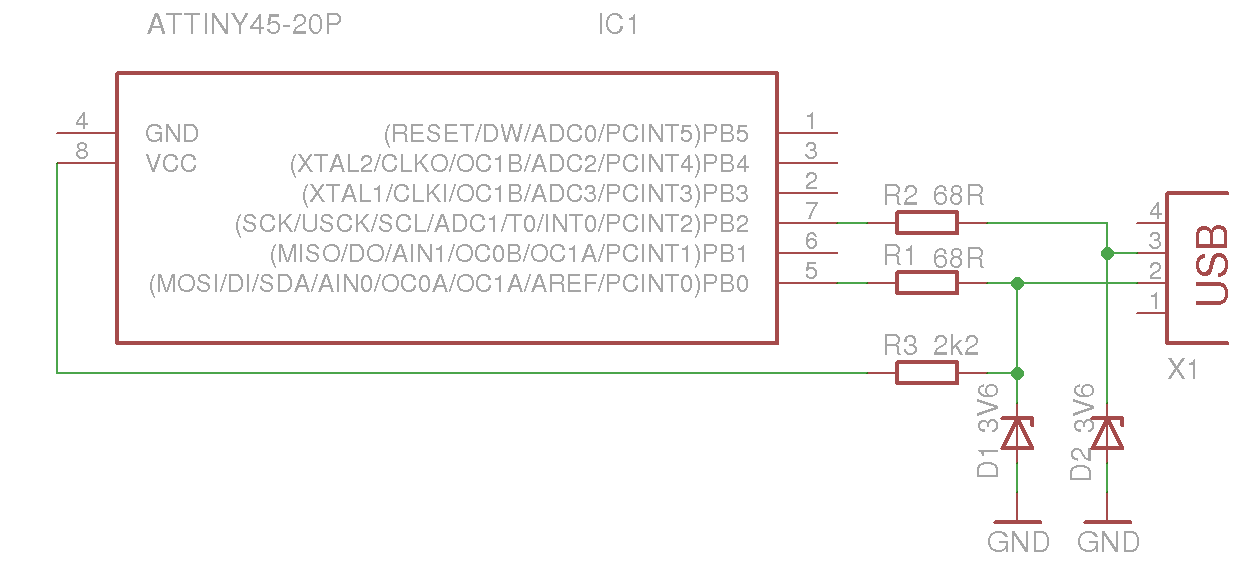
\includegraphics[width=\textwidth]{afbeeldingen/circuit_signaal}
	\caption{Signaalconversie}
\end{figure}

\subsection{\acs{isp}}

Het invoegen van een \ac{isp} header is niet veel werk: we dienen gewoon te voorzien in een connector, en de pinnen ervan correct doorverbinden met de juiste pinnen van de microcontroller.

TODO: programmeren als systeem actief is?

\begin{figure}
	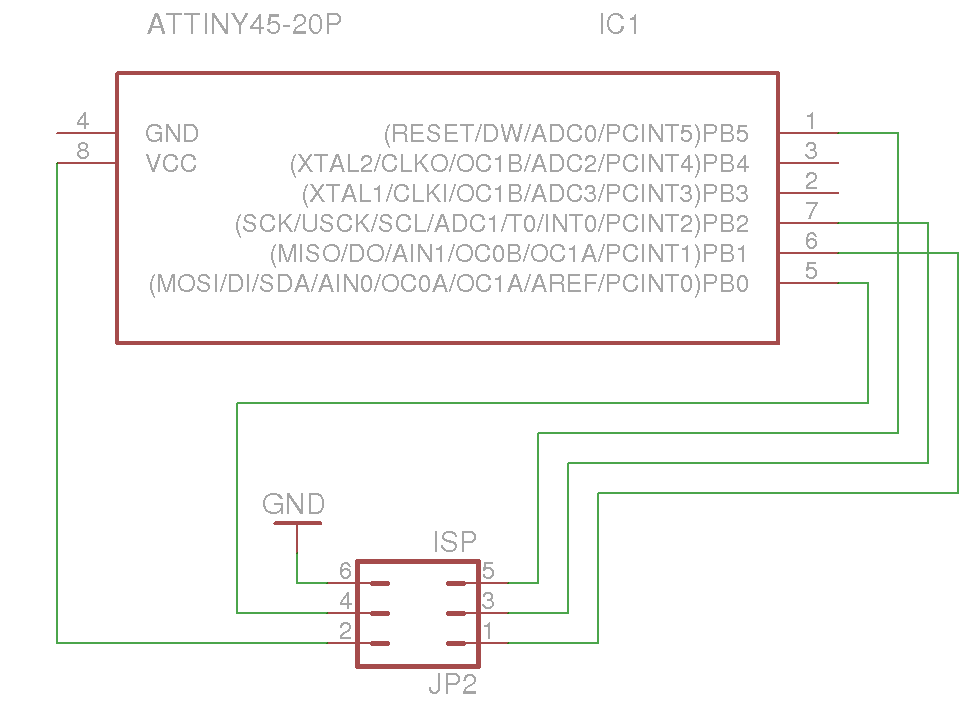
\includegraphics[width=\textwidth]{afbeeldingen/circuit_isp}
	\caption{\acs{isp} connector}
\end{figure}

\section{Schakelaars}

De schakelaars bevinden zich fysiek niet op de interface module, maar zijn reeds ingebouwd in de bestaande kasten. Daarom zullen we een systeem moeten bedenken om de bestaande schakelaars op een handige manier op de module aan te sluiten. Tevens moeten we de knoppen zodanig verbinden dat er uitbreidingsmogelijkheden zijn.

Om de bestaande schakelaars op een eenvoudige manier aan te sluiten, zullen we de interface module voorzien van een connector waarop we eenvoudig knoppen kunnen op aansluiten. De meest robuuste oplossing hierbij is een connector die vastklikt op de module, waardoor die niet per toeval kan loskomen. Dergelijke connectors zijn echter vrij specifiek, en vereisen per aan te sluiten schakelaar een element op de printplaat. Een alternatief, dat als voordeel heeft dat het geen speciale connector aan de kant van de knoppen vereist, zijn vijs-connectors. Hierbij worden de losse draden van de knoppen via een vijsaansluiting op de printplaat bevestigd. Hoewel dit al een betere oplossing is, vereist het nog altijd een connector op de printplaat voor elke knop, en neemt het vast- en losvijzen van de kabels ook meer tijd in beslag dan het aansluiten van een eenvoudige connector. Daarom hebben we gekozen voor de alombekende \emph{jumpers}. Deze makkelijk te vinden connectors kunnen eenvoudig aan het kabelpaar van de knoppen bevestigd worden door middel van een krimptang. Aan de kant van de printplaat is het ook een eenvoudigere oplossing, daar het mogelijk is de aansluitingen voor alle schakelaars door middel van een enkel blok jumpers te realiseren. Het enige nadeel is dat een aangesloten connectors niet zo vast zitten: bij gebrek aan weerhaak of ander systeem kan de kabel relatief gemakkelijk loskomen.

Om de aansluitingen op de printplaat eenvoudig te houden, zullen we werken met een \emph{active-low} mechanisme: een knop zal wanneer ingedrukt bepaalde signaallijnen doorverbinden met de elektrische grond. Om er voor te zorgen dat er een hoog signaal gemeten wordt wanneer er geen verbinding is met de elektrische grond, maken we gebruik van de interne pull-up die beschikbaar is voor elke poortpin: dit is een weerstand tussen de $20$ en $50$ kilo-ohm die de poortpin intern doorverbindt met de positieve voedingslijn. Hierdoor zal bij afwezigheid van een externe verbinding de spanning op de poortpin gelijk zijn aan de voedingsspanning, wat gedetecteerd wordt als een hoog signaal. Wanneer we echter de poortpin zullen doorverbinden naar de elektrische grond, zal deze pull-up weerstand zorgen voor een stroom tussen de $0.1$ en $0.25$ milliampères.

Er is echter een bijkomend probleem: we hebben maar 3 poortpinnen tot onze beschikking, waardoor het niet mogelijk is elke knop door te verbinden met een eigen poortpin. De eenvoudige oplossing hierbij is het gebruik van een multiplexer: 2 select-lijnen en 1 datalijn maakt het mogelijk om 4 schakelaars uit te lezen. We willen echter meer knoppen kunnen aansluiten, zonder daarbij extra poortpinnen nodig te hebben. Daarom zullen we zelf het signaal multiplexen, waarbij we meer schakelaars kunnen toelaten door geen gebruik te maken van een selectiemechanisme, maar de signalen direct door te linken naar de poortpinnen. Het nadeel aan deze opzet is dat de signalen kunnen overlappen, zo zullen we bij het indrukken van meerdere knoppen tegelijkertijd niet kunnen uitmaken welke knoppen juist ingedrukt zijn.

De realisatie van een dergelijke multiplexer lijkt eenvoudig, maar er is een belangrijk detail dat we moeten opmerken. Aangezien de verschillende poortpinnen verbonden zijn met verschillende knoppen, kan er bij het indrukken van een enkele schakelaar stroom terugvloeien via de contactpunten van diens signaallijnen met andere knoppen van een totaal ongerelateerde poortpin, zoals te zien is op figuur \ref{fig:circuit_schakelaars_foutief}. Om dit te vermijden moeten we overal waar er twee signaallijnen met elkaar verbonden zijn, een diode plaatsen zodat er geen stroom kan terugvloeien naar een vorig verbindingspunt. Hiervoor hebben we een reguliere diode nodig, waarbij geen speciale eisen gesteld worden. Daarom kiezen we voor de 1N4148, een populaire diode die vaak gebruikt wordt voor het schakelen van digitale signalen. Zoals we kunnen opzoeken in het stroom-spanningsdiagram van deze diode, zorgt ze bij een stroom tussen $0.1$ en $0.25$ milliampères (gegenereerd door de pull-up weerstand binnen de microcontroller) voor een spanningsval van $0.5$ volt.

\begin{figure}
	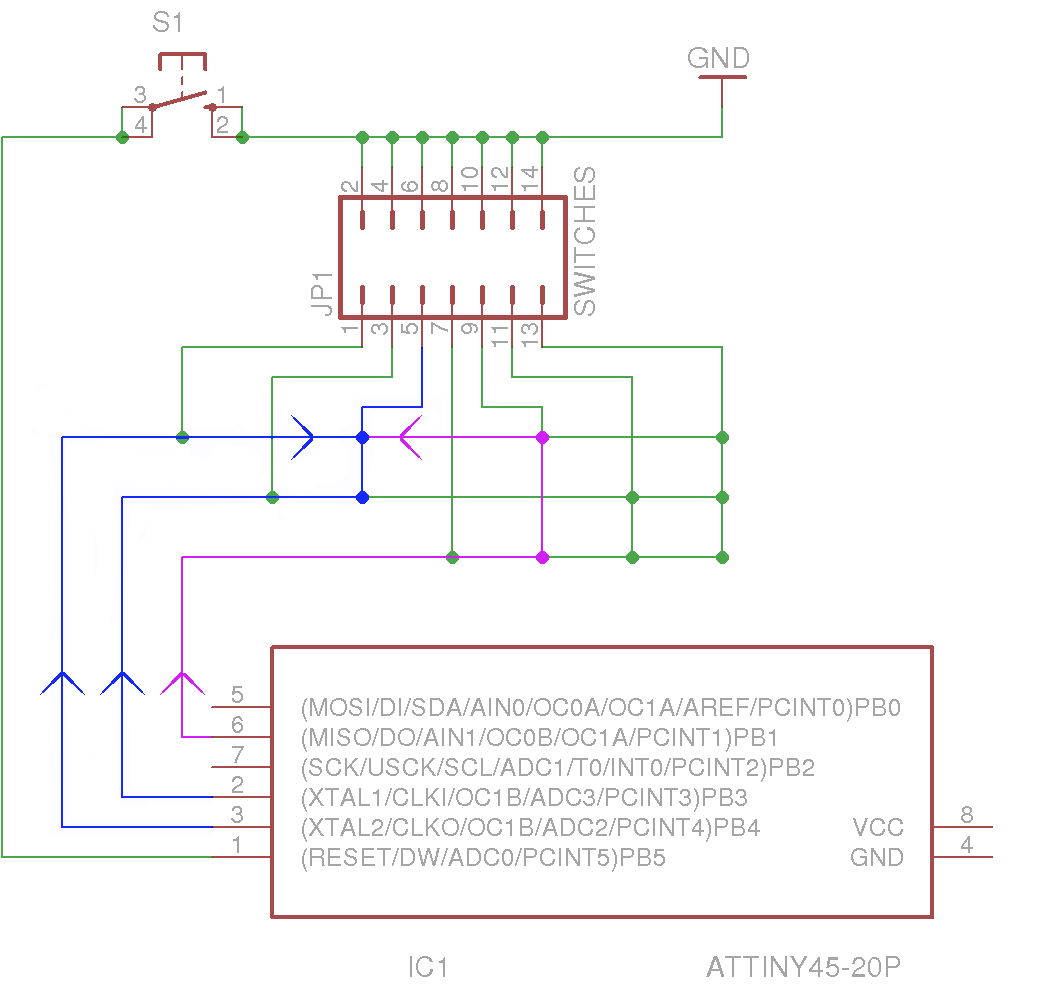
\includegraphics[width=\textwidth]{afbeeldingen/circuit_schakelaars_foutief}
	\caption{Circuit en connector voor schakelaars zonder dioden, en aanduiding van voorbeeldstromen daarbij}
	\label{fig:circuit_schakelaars_foutief}
\end{figure}

We kunnen wel niet zomaar dioden op de signaallijnen plaatsen. Als we dit wel zouden doen, zou de het volledige spanningsverschil tussen de elektrische grond en de poortpin (wat $5$ volt bedraagt, dankzij de interne pull-up) over de diode geplaatst worden, waardoor die beschadigd zou worden. Dit zou opgelost kunnen worden door bij elk van de drie poortpinnen een extra beschermingsweerstand te plaatsen, waardoor de overmatige spanning over deze weerstand zou komen te staan en de dioden slechts het spanningsverschil waarvoor ze gemaakt zijn zouden moeten verwerken. Het berekenen van de waarde van deze weerstand zou wel enig werk vereisen, daar we moeten zorgen dat de spanning die aan het hoogimpedant meetcircuit aangelegd wordt zich binnen het bereik van een laag signaal bevindt. De datasheet van de microcontroller stelt zo dat een laag signaal gedetecteerd wordt tussen $0$ volt en $0.6$ keer de bronspanning. Aangezien de microcontroller zich rechtstreeks voedt met de USB bronspanning, dewelke $5$ volt bedraagt, moet de spanning aan het meetcircuit vallen tussen $0$ en $3$ volt.

Als we echter nauwkeuriger kijken naar de werking van de interne pull-up (figuur \ref{fig:avr_pullup}), zien we dat deze reeds op zichzelf functioneert als een beschermingsweerstand. In het slechtste geval bijvoorbeeld, waarbij er zich na de pull-up nog drie dioden met elk een spanningsval van $0.5$ volt bevinden, zal er zich zo slechts $1.5$ volt op de signaallijn bevinden, wat ruim binnen de grenzen voor detectie van een laag signaal bevindt. Aangezien de weerstand tevens voldoende groot is, moeten we niet zorgen voor een extra stroomreductie en verdwijnt elk nut van een extra beschermingsweerstand.

\begin{figure}
	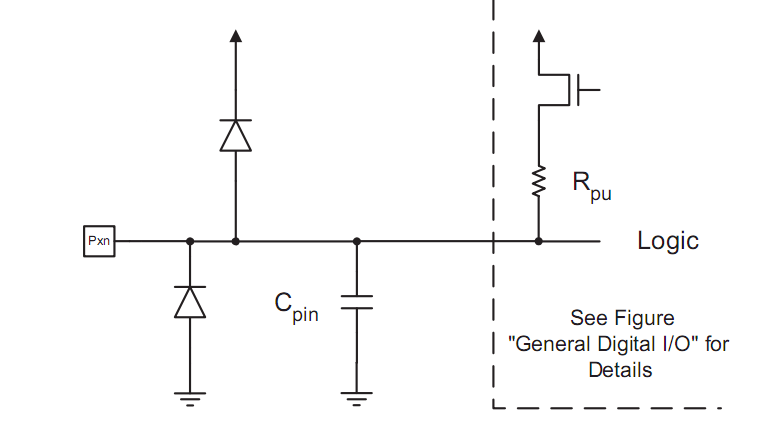
\includegraphics[width=\textwidth]{afbeeldingen/avr_pullup}
	\caption{Pull-up weerstand binnenin een AVR microcontroller}
	\label{fig:avr_pullup}
\end{figure}

\begin{figure}
	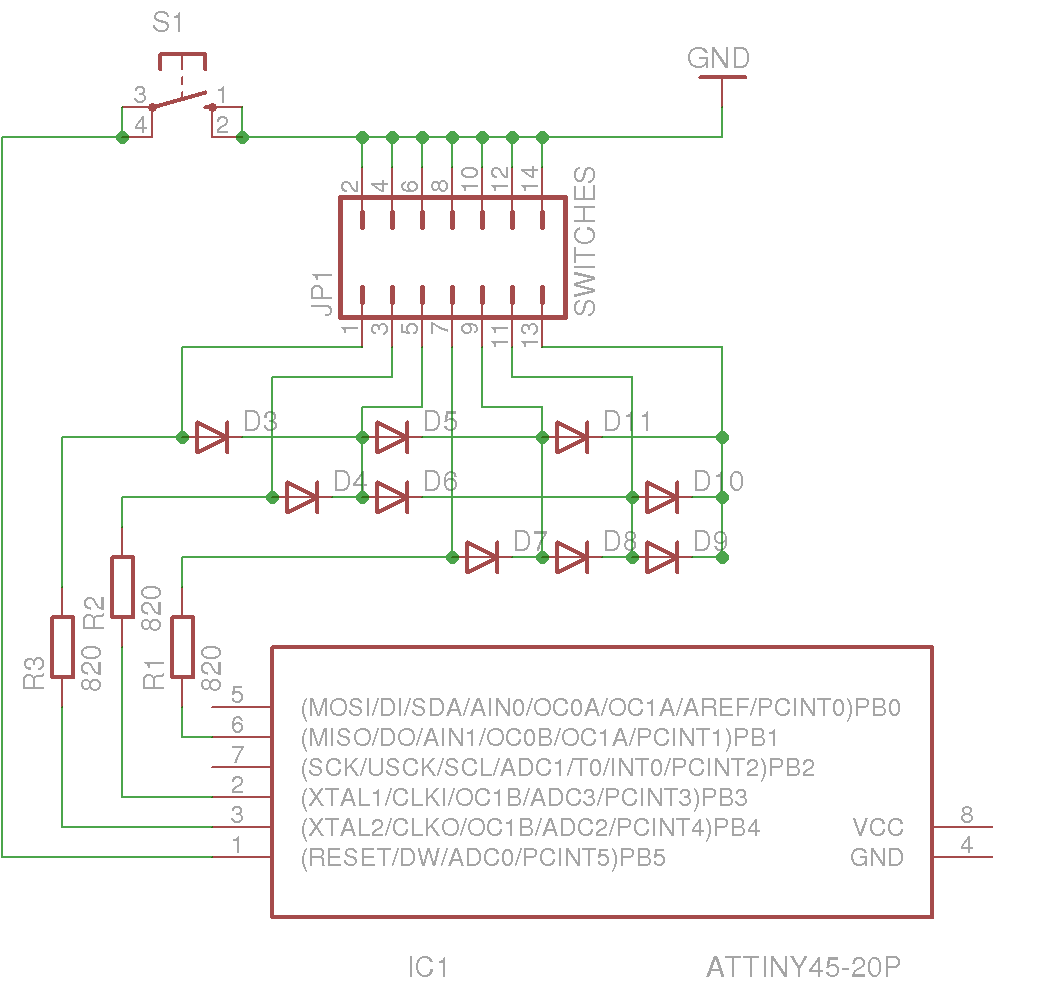
\includegraphics[width=\textwidth]{afbeeldingen/circuit_schakelaars}
	\caption{Circuit en connector voor schakelaars}
\end{figure}

\begin{figure}
	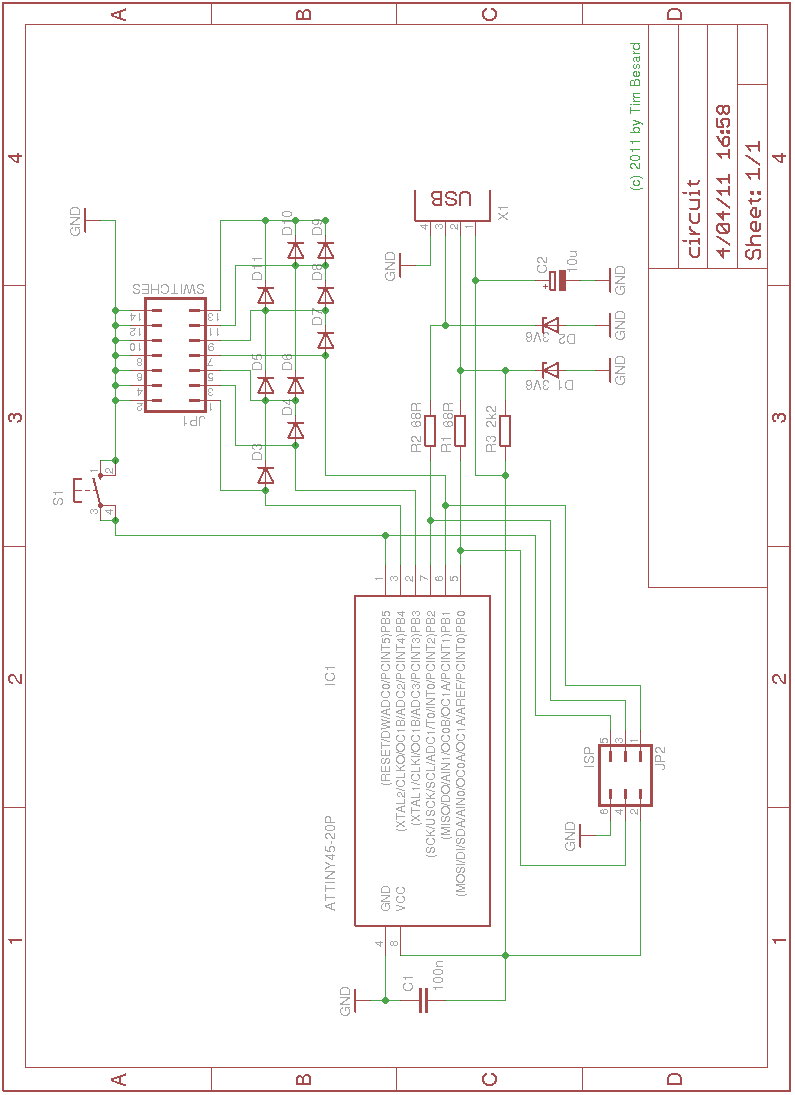
\includegraphics[width=\textwidth]{afbeeldingen/circuit}
	\caption{Uiteindelijk circuit}
\end{figure}

\section{Productie}

De finale stap bestaat eruit om het ontworpen schema te realiseren en een fysieke printplaat te laten maken, ofte een \ac{pcb}. Hierbij moeten we manueel een fysieke layout aanmaken en baantjes trekken waar er stroom moet kunnen vloeien. De plaatsing van die componenten is echter niet louter willekeurig. Zo is het bijvoorbeeld interessant om de componenten efficiënt te plaatsen zodat de uiteindelijke printplaat zo klein mogelijk is. Maar er zijn ook andere zaken waarmee we moeten rekening houden. Zo is er bijvoorbeeld de kwestie van plaatsing van de ontkoppelingscondesatoren: die worden best zo dicht mogelijk bij de bron van de spanningsoscillaties geplaatst.

Vooraleerst zijn we op zoek gegaan naar een fabrikant die voor een aanvaardbaar tarief een voldoende gesofisticeerde printplaat kan produceren. De mogelijkheden zijn eens te meer zeer uitgebreid, maar na een uitgebreide vergelijking zijn we terechtgekomen bij \makeurl{http://www.eurocircuits.com/}{Eurocircuits}, een Europees bedrijf met verschillende vestigingen, waaronder België. Hoewel de verschillen tussen andere fabrikanten niet al te groot zijn, heeft de combinatie van een competitieve prijs, beperkte verzendkosten, en verschillende positieve kritieken ons ertoe overtuigd om voor de diensten van Eurocircuits te kiezen.

Vervolgens hebben we een gekeken naar de eisen en mogelijkheden die het goedkoopste van de productietypes te vinden bij Eurocircuits - de standard pool - biedt. De \makeurl{http://www.eurocircuits.com/images/stories/ec09/ec-standard-pool-overview-english-1-2010-v3.pdf}{volledige lijst} is te uitgebreid om hier te vermelden, daarom halen we enkel de belangrijkste elementen aan:
\begin{itemize}
\item Maximaal 8 layers;
\item Top- en bottom solder mask;
\item Top- en bottom silkscreen.
\end{itemize}
Om de overige eisen, denk maar aan de minimale afstand tussen boorgaten of de minimale breedte van elektrische baantjes, te controleren zullen we gebruik maken van een \ac{dru} bestand. Dergelijke bestanden worden vaak aangeboden door te fabrikant, en laten toe om geautomatiseerd alle eisen te controleren die aan een printplaat gesteld worden.

Om een printplaat of printplaat te ontwerpen hebben we natuurlijk gepaste software nodig. De meest populaire keuze hierbij is de EAGLE PCB software, ontwikkeld door \makeurl{http://www.cadsoftusa.com/}{CadSoft}, waarschijnlijk omdat er een beperkte variant van de software gratis beschikbaar is. Wegens de populariteit van de tool bestaat er een heel actieve community, waardoor een zeer uitgebreide selectie aan componenten beschikbaar zijn voor gebruik binnen EAGLE. Ook biedt Eurocircuits enkel \ac{dru} bestanden aan voor de EAGLE software. Het lijkt daarom een verstandige keuze om onze printplaat ook te ontwerpen met EAGLE.

Nu we alle nodige specificaties vergaard hebben en een softwarepakket geselecteerd hebben, kunnen we beginnen aan het produceren van de fysieke layout. Hierbij hebben we ervoor gekozen om een printplaat te maken die bestaat uit twee lagen, namelijk de boven en onderkant. Deze optie is niet veel duurder dan een 1-laags printplaat, en het geeft ons de nodige flexibiliteit om de componenten goed te kunnen plaatsen. Moesten we gekozen hebben voor een 1-laags printplaat dan zou de kost misschien zelfs hoger kunnen liggen door soms onnatuurlijke plaatsing om toch de nodige verbindingen te kunnen realiseren.

\begin{figure}
	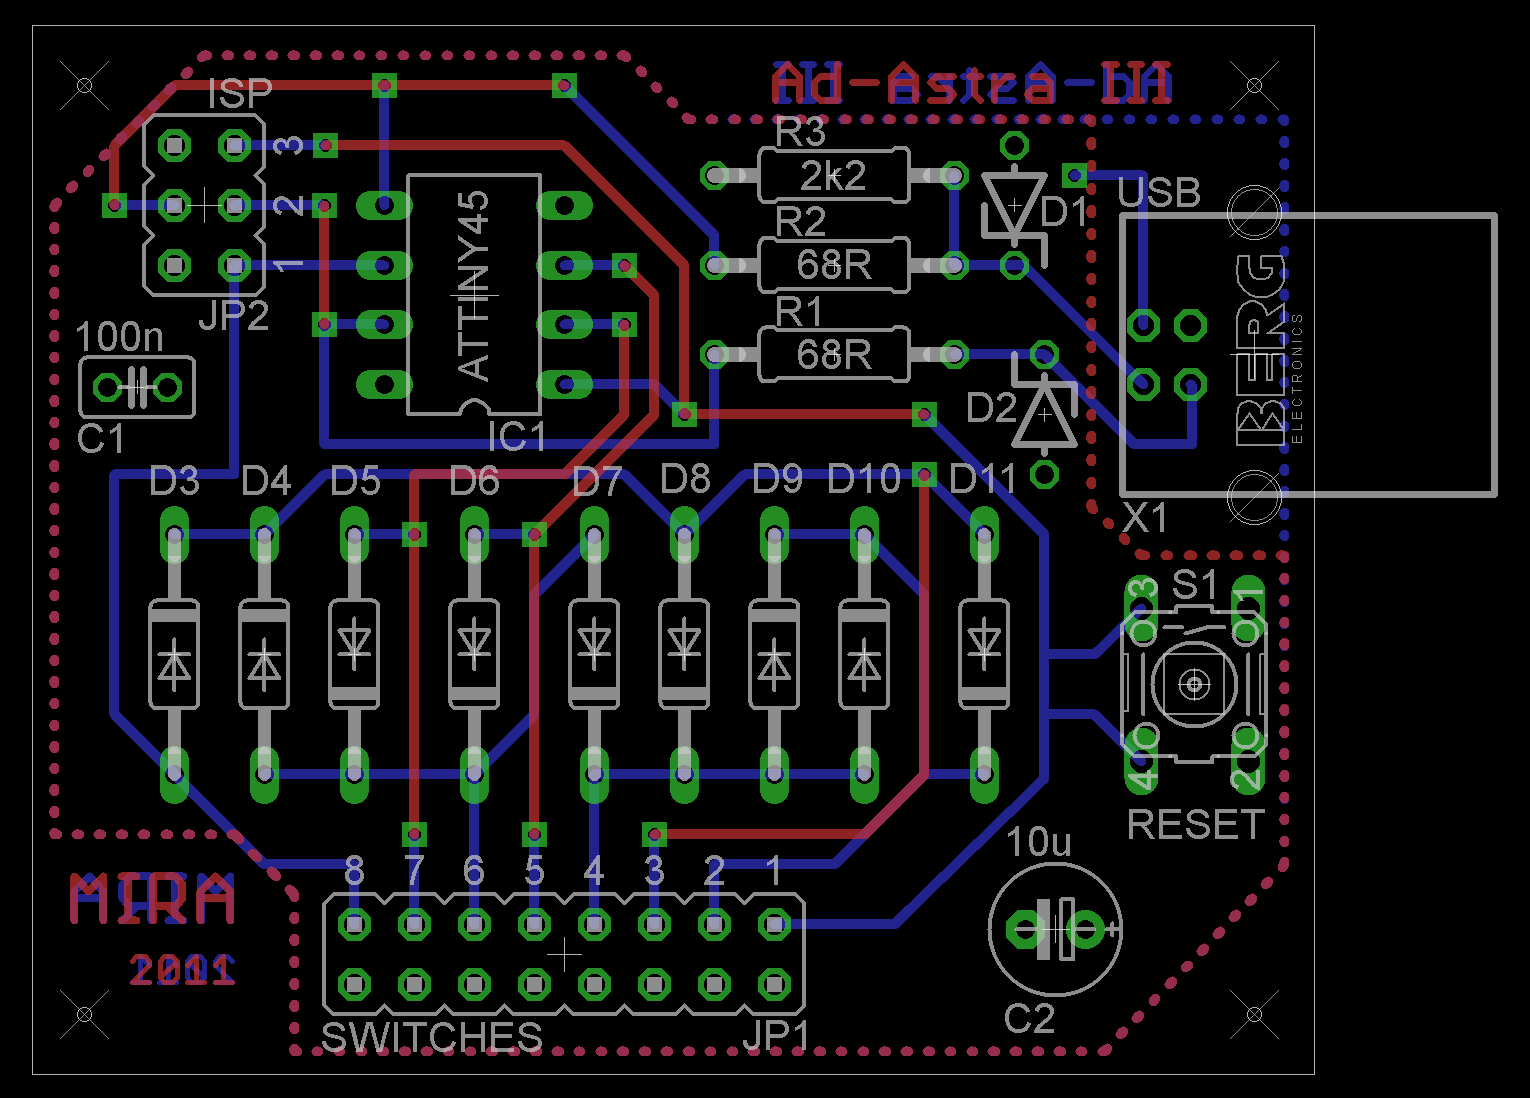
\includegraphics[width=\textwidth]{afbeeldingen/circuit_pcb}
	\caption{Finale versie van de printplaat}
\end{figure}

\begin{figure}
	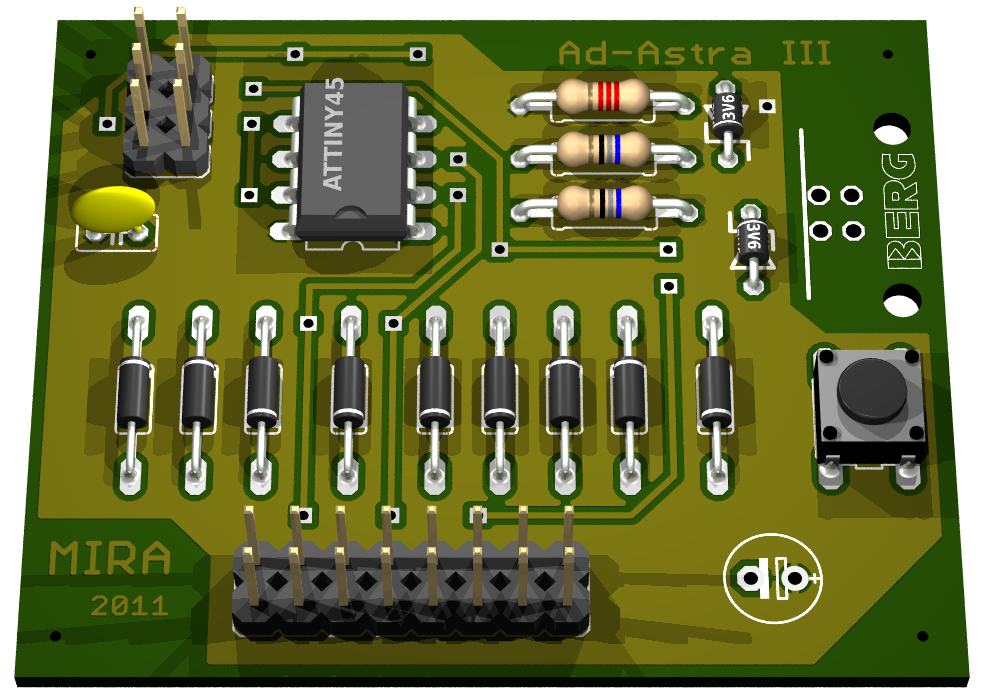
\includegraphics[width=\textwidth]{afbeeldingen/circuit_pcbrender}
	\caption{3D-render van de printplaat}
\end{figure}


\chapter{Firmware}

\end{document}


\part{Invoering}
\label{invoering}

\textit{Dummy tekst omdat \LaTeX anders zot komt.}


\chapter{Conclusie}

% todo: mag niet teveel op abstract lijken
% http://www.dissertationswriting.co.uk/dissertation_conclusion.htm 

Het doel van deze thesis was de ontwikkeling van een modern multimediaframework dat zorgt voor de opslag, distributie en weergave van multimediafragmenten op de kiosken van de volkssterrenwacht MIRA. Daarbij is belangrijk dat een beheerder elk van die processen voldoende kan opvolgen en beïnvloeden, zonder al teveel technische kennis nodig te hebben. Ook moet het mogelijk zijn om mooie voorstellingen te realiseren met de middelen die het platform aanbiedt, en tegelijk compatibel te zijn met de voorstellingen die momenteel gebruikt worden.

We hebben ervoor gekozen om de voorstellingen op te maken in \ac{html} en Javascript, waarmeer we zeer rijke gebruikerservaringen kunnen ontwerpen. Ook compatibiliteit met de huidige voorstellingen is ermee mogelijk: na conversie naar het WebM formaat kunnen we de fragmenten gebruiken binnen \ac{html}. Om daarbij dynamisch de taalkeuze van de gebruiker in te verwerken hebben we voorzien in een kleine webapplicatie, opgebouwd met behulp van JQuery.
Vervolgens worden de voorstellingen opgeslaan in een \ac{svn} repository, waardoor efficiënte overdracht bekomen wordt en een beheerder relatief eenvoudig wijzigingen kan doorvoeren aan de inhoud van de voorstellingen.

% server

% client

% inputmodule

% conclusie

% Bibliografie
\bibliographystyle{plainnat}
\bibliography{verslag}


\end{document}
